\documentclass[notes, aspectratio=1610]{beamer}
%\documentclass[aspectratio=1610]{beamer}

% =================================== Colors ================================
\definecolor{base_c}{rgb}{
	0.1411764705882353, 0.6235294117647059, 0.33725490196078434
	}
\definecolor{comp_c}{rgb}{
	0.6235294117647059, 0.1411764705882353, 0.42745098039215684
	}
\definecolor{tri_1}{rgb}{
	0.33725490196078434, 0.1411764705882353, 0.6235294117647059
	}
\definecolor{tri_2}{rgb}{
	0.6235294117647059, 0.33725490196078434, 0.1411764705882353
	}
\definecolor{white}{rgb}{1,1,1}
\usepackage{color, colortbl}

% ================================ Text boxes ==============================
\usepackage[most]{tcolorbox}

% ================================ Symbols ==============================
%\usepackage{bbding}
%\usepackage{pifont}
%\usepackage{wasysym}
%\usepackage{amssymb}

% ========================= Theme =========================================
\usetheme{Berkeley}
\usecolortheme{spruce}
% \setbeamercolor{itemize item}{fg=comp_c,bg=white}
% \setbeamercolor{enumerate item}{fg=comp_c,bg=white}

% ========================= Essential packages ============================
% \usepackage{hyperref}
% \hypersetup{
%     colorlinks = false,
%     linkcolor = comp_c,
%     citecolor = tri_1,
%     filecolor = tri_2,
%     urlcolor = yellow
% }

% ========================= Frame notes systm ============================
%\usepackage{pgfpages}
%\setbeameroption{show notes on second screen}

% ========================= Plotting ======================================
\usepackage{calc}
\usepackage{tikz}
\usetikzlibrary{arrows,
                arrows.meta,
                calc,
		chains,
                quotes,
                positioning,
		shapes,
		topaths,
                shapes.geometric}
\usepackage{graphicx}
\usepackage{graphics}
\usepackage{pgfplots}
\pgfplotsset{width=7cm,compat=1.17}
\usepackage{venndiagram}
% tikz exhibits
\usepackage{tikz}
\usetikzlibrary{shapes,arrows,fit,calc,positioning}
\tikzstyle{box} = [draw, rectangle, rounded corners, thick, node distance=7em, text width=6em, text centered, minimum height=3.5em]
\tikzstyle{container} = [draw, rectangle, dashed, inner sep=2em]
\tikzstyle{lineSq} = [draw, thick, -latex']
\tikzset{
	%Define standard arrow tip
	>=stealth',
	%Define style for boxes
	punkt/.style={
	       rectangle,
	       rounded corners,
	       draw=black, thick,
	       text width=8em,
	       minimum height=3em,
	       text centered},
	punkbig/.style={
		   rectangle,
		   rounded corners,
		   draw=black, thick,
		   text width=5em,
		   minimum height=5em,
		   text centered},
	punkb/.style={
		   rectangle,
		   rounded corners,
		   %draw=black, thick,
		   text width=8em,
		   minimum height=3em,
		   text centered},
	punkc/.style={
	       circle,
	       rounded corners,
	       draw=black, thick,
	       text width=1.5em,
	       minimum height=1.5em,
	       text centered},
	% Define arrow style
	pil/.style={
	       ->,
	       thick,
	       shorten <=2pt,
	       shorten >=2pt,}
}

% ============================= Network viz ===============================
\usepackage{tikz-network}

%% ============================== Tabular =================================
\usepackage{booktabs}
\usepackage{tabularx,ragged2e}
\usepackage{array}
\usepackage{multirow}
\usepackage{siunitx}
  \sisetup{detect-all}
\usepackage{adjustbox}
\usepackage{rotating}
\usepackage{threeparttable}
\usepackage[justification=centering]{caption}

%% ========================== Coding snippets =============================
% Default fixed font does not support bold face
%\usepackage{minted}
%\usemintedstyle{vs}

%% ============================= Math =====================================
\usepackage{mathtools}

% ========================= Infor on authors ==============================
\title[Networks and Value Creation]
{When Do Networks Create Value?}
\subtitle{Bonding Social Capital and Centrality}
\author{S.~Santoni\inst{1}\inst{2}}
\institute{
	\inst{1}%
	Bayes Business School
	\and
	\inst{2}%
	Soundcloud
	}
\date{MSc in Business Analytics, 2022/23}

% ========================= TOC  ==========================================
\AtBeginSection[]
{
	\begin{frame}
		       \frametitle{Outline}
		       \tableofcontents[currentsection,currentsubsection]
	\end{frame}
}

% ========================= References ===================================
\usepackage[style=numeric,backend=biber]{biblatex}
\addbibresource{bibliography.bib}

% =========================== TOC =========================================
\AtBeginSubsection[]
{
    \begin{frame}
        \frametitle{Outline}
        \tableofcontents[currentsection,currentsubsection]
    \end{frame}
}

% ========================= Document  ====================================
\begin{document}

\begin{frame}
	\titlepage
\end{frame}

\begin{frame}{Outline}
	\tableofcontents
\end{frame}

% =========================== Session 2 wrapup =============================
\section{Session 2 Wrap Up}

\begin{frame}
\tikzstyle{block} = [
	rectangle, 
	draw,
	text width=8em,
	text centered,
	rounded corners,
	minimum height=2em
	]
\tikzstyle{arrow} = [
	draw,
	-latex',
	rounded corners
	]
\tikzstyle{line} = [
	draw
	]
\tikzstyle{invisible4} = [
	rectangle
	]
\tikzstyle{invisible5} = [
	rectangle
	]
	\frametitle{Where Does a Network Analytics Project Stand?}
	\begin{figure}
		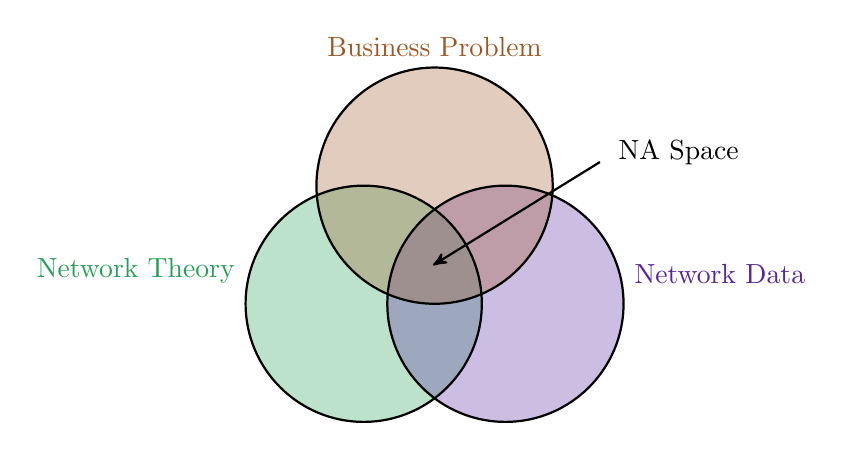
\begin{tikzpicture}[
			thick,
			set/.style = {circle, minimum size = 3cm, opacity=0.3},
			auto,
			->,
			]
			\node[set,label={[text=base_c]175:Network Theory}, fill=base_c] (A) at (0,0) {};
		 	\node[set,label={[text=tri_1]5:Network Data}, fill=tri_1] (B) at (1.8,0) {};
		 	\node[set,label={[text=tri_2]Business Problem}, fill=tri_2] (C) at (0.9,1.5) {};
		  	% circles
		  	\draw (0,0) circle(1.5cm);
	    	 	\draw (1.8,0) circle(1.5cm);
	     	        \draw (0.9,1.5) circle(1.5cm);
			% notes 
			\node[,label={[text=black]NA Space}] (i2) at (4,1.5) {};
			\node[] (p2) at (0.75,0.49) {};
			% edges 
			\path[]
			(3,1.8) edge[bend right=0] node [] {} (p2.east)
			;
		\end{tikzpicture}
	\end{figure}	
\end{frame}

\begin{frame}
	\frametitle{Real World Problem Statements I Worked With}
	\begin{quote}
		``Our data say employees have not come up with 
		fresh ideas for quite a while. We need to find out.''
	\end{quote}
	\raggedleft --- The innovation platform manager of a global public utility.

	\vspace{1em}

	\begin{quote}
		``The people in the [R\&D] department do not part-take in 
		the decision making process regarding the selection 
		of the future projects. Shall they?''
	\end{quote}
	\raggedleft --- The Head of Reserch of a big pharma company.
	\vspace{1em}

	\begin{quote}
		``Engineers want more autonomy in forming a new product 
		development team. What are the pros and cons?''
	\end{quote}
	\raggedleft --- The CTO of a global semiconductor company.
\end{frame}

\begin{frame}
	\frametitle{Mapping Business Problems on Objective Functions and Domains}
	\begin{table}
		\begin{small}
			\begin{center}
				\begin{tabular}[c]{
					p{3cm}|p{2.1cm}|p{2.1cm}|p{2.1cm}|p{2.1cm}
					}
					%\hline
					\multicolumn{1}{c}{\textbf{}}
					& \multicolumn{4}{c}{\textbf{Domain}}\\
					\hline
					\textbf{Objective function}
					&\multicolumn{1}{c|}{\textbf{Employee}}
					&\multicolumn{1}{c|}{\textbf{Project}}
					&\multicolumn{1}{c|}{\textbf{Organization}}
					&\multicolumn{1}{c}{\textbf{Inter-orgs}}\\
					\hline
					Creativity\dotfill&
					\cellcolor{white!25}\multicolumn{1}{c}{\bullet}& 
					\cellcolor{white!25}\multicolumn{1}{c}{\bullet}&
					&
					\\ 
					% \cline{2-5}
					Knowledge sharing\dotfill&
					\cellcolor{white!25}\multicolumn{1}{c}{\bullet}&
					\cellcolor{white!25}\multicolumn{1}{c}{\bullet}&
					&
					\\
					% \cline{2-5}
					Task performance\dotfill&
					\cellcolor{white!25}\multicolumn{1}{c}{\bullet}&
					\cellcolor{white!25}\multicolumn{1}{c}{\bullet}&
					&
					\\ 
					Coordination\dotfill&
					\cellcolor{white!25}\multicolumn{1}{c}{\bullet}&
					\cellcolor{white!25}\multicolumn{1}{c}{\bullet}&
					\cellcolor{white!25}\multicolumn{1}{c}{\bullet}&
					\cellcolor{white!25}\multicolumn{1}{c}{\bullet}\\
					% \cline{2-5}
					Innovation\dotfill&
					\cellcolor{white!25}\multicolumn{1}{c}{\bullet}&
					\cellcolor{white!25}\multicolumn{1}{c}{\bullet}&
					\cellcolor{white!25}\multicolumn{1}{c}{\bullet}&
					\cellcolor{white!25}\multicolumn{1}{c}{\bullet}\\ 
					% \cline{2-5}
				        Econ performance\dotfill&
					&
					&\cellcolor{white!25}\multicolumn{1}{c}{\bullet}
					&
					\\
					% \hline
				\end{tabular}
			\end{center}
		\end{small}
	\end{table}
	\textit{Notes.} --- The table shows common associations between business problems' 
	objective functions (what clients want to achieve in essence) 
	and domains (the level at which the problem should be addressed). Dots 
	denote the existence of common associations.
\end{frame}

\begin{frame}
	\frametitle{Forms of Networks}
	It is socially accepted to distinguish networks between

	\begin{itemize}
		\item 
   		Directed Vs undirected
		\item
   		Weighted Vs unweighted
		\item  		
		One Vs two-mode
	\end{itemize}
	
	\vspace{1em}

	\begin{tcolorbox}[
		colback=comp_c!5!white,
		colframe=comp_c!90!black,
		title={\centering !! Pay attention !!}]
		These categories are not mutually exclusive. E.g., a network can be 
		both directed and weighted.
	\end{tcolorbox}
	
\end{frame}

\begin{frame}
	\frametitle{The Goals of Network Theory}
	Mainly, network theory aims to explain
	\begin{enumerate}
		\item Why some nodes or groups achieve more (the 
		social capital tradition)
		\item Why some nodes or  networks  are  more  similar  to  
		each  other  (the  social   homogeneity   tradition)
	\end{enumerate}
\end{frame}

\begin{frame}
	\frametitle{Network Theory's Network Views}

	Network theories mirror two different views of networks

	\begin{itemize}
		\item The first view --- known as the `network flow model' 
		--- emphasizes the information, resources, or artefacts 
		that flow through the network and possibly accrue to 
		the individual nodes
		\begin{itemize}
			\item \textit{Sample proposition}: central nodes have an information advantage
			over peripheral ones
		\end{itemize}
		\item The second view --- known as the `network architecture 
		model' --- highlights the connection between network structure 
		and individual or organizational outcomes  
		\begin{itemize}
			\item \textit{Sample proposition}: decentralized organizational 
			structures are more suited in high-tech industries than
			low-tech companies
		\end{itemize}
	\end{itemize}
\end{frame}

\begin{frame}
	\frametitle{Groups of Network Theories}
	\centering
	\small
	\begin{table}
		\begin{center}
			\begin{tabular}[c]{l|l|l}
				% \hline
				\textbf{Underlying model} & 
				\textbf{Social capital} &
				\textbf{Social homogeneity}\\
				\hline
				\textbf{Network flow} & Capitalization (value creation) & Contagion  \\
				\hline
				\textbf{Network architecture} & Coordination & Adaptation  (network change)\\
				% \hline
			\end{tabular}
		\end{center}
	\end{table}

	\vspace{1em}

	\raggedright \small Source is~\cite[][page 47]{scott2011}
\end{frame}

% =========================== Session 3 ===================================
\section{When Do Networks Create Value?}

\begin{frame}
	\frametitle{Groups of Network Theories}
	\centering
	\small
	\begin{table}
		\begin{center}
			\begin{tabular}[c]{l|l|l}
				% \hline
				\textbf{Underlying model} & 
				\textbf{Social capital} &
				\textbf{Social homogeneity}\\
				\hline
				\textbf{Network flow} & \cellcolor{blue!20}{\color{black}{Capitalization (value creation)}} & Contagion  \\
				\hline
				\textbf{Network architecture} & Coordination & Adaptation  (network change)\\
				% \hline
			\end{tabular}
		\end{center}
	\end{table}

	\vspace{1em}

	\raggedright \small Source is~\cite[][page 47]{scott2011}
\end{frame}

\begin{frame}
	\frametitle{The Leading Question}
		\begin{center}
			\LARGE When do networks create value?
		\end{center}
\end{frame}

\begin{frame}{Theories on Networks and Value Creation}
\begin{columns}
	\begin{column}{0.5\textwidth}
	Mainly, the various theories on the influence of networks on value 
	creation can be grouped into two categories:

	\vspace{1em}

	\begin{itemize}
		\item \textbf{Bridging} social capital theories, whose key 
		      tenet is that sparse networks bring value to 
		      individuals and groups by facilitating fresh courses 
		      of action and new ideas --- a process called 
		      \textbf{network brokerage} 
		\item \textbf{Bonding} social capital theories, whose key 
		      tenet is that dense networks bring value to 
		      individuals and groups by fostering cooperation and trust
		      ---  a process called \textbf{network closure}
	\end{itemize}
	\end{column}
	\begin{column}{0.5\textwidth}
		\centering
		
\includegraphics[width=0.75\textwidth]{images/brokerage_and_closure.jpeg}
	\end{column}
\end{columns}
\end{frame}

% =========================== Bonding Social Capital ======================= 
\section{Bonding Social Capital and Value Creation}

\begin{frame}{Today's Class Focus}
\begin{columns}[c]
	\begin{column}{0.5\textwidth}
	\Large The attention revolves around the topic of \textcolor{base_c}{
		bonding social capital} and the \textcolor{comp_c}{closure 
		mechanism}
	\end{column}
	\begin{column}{0.5\textwidth}
		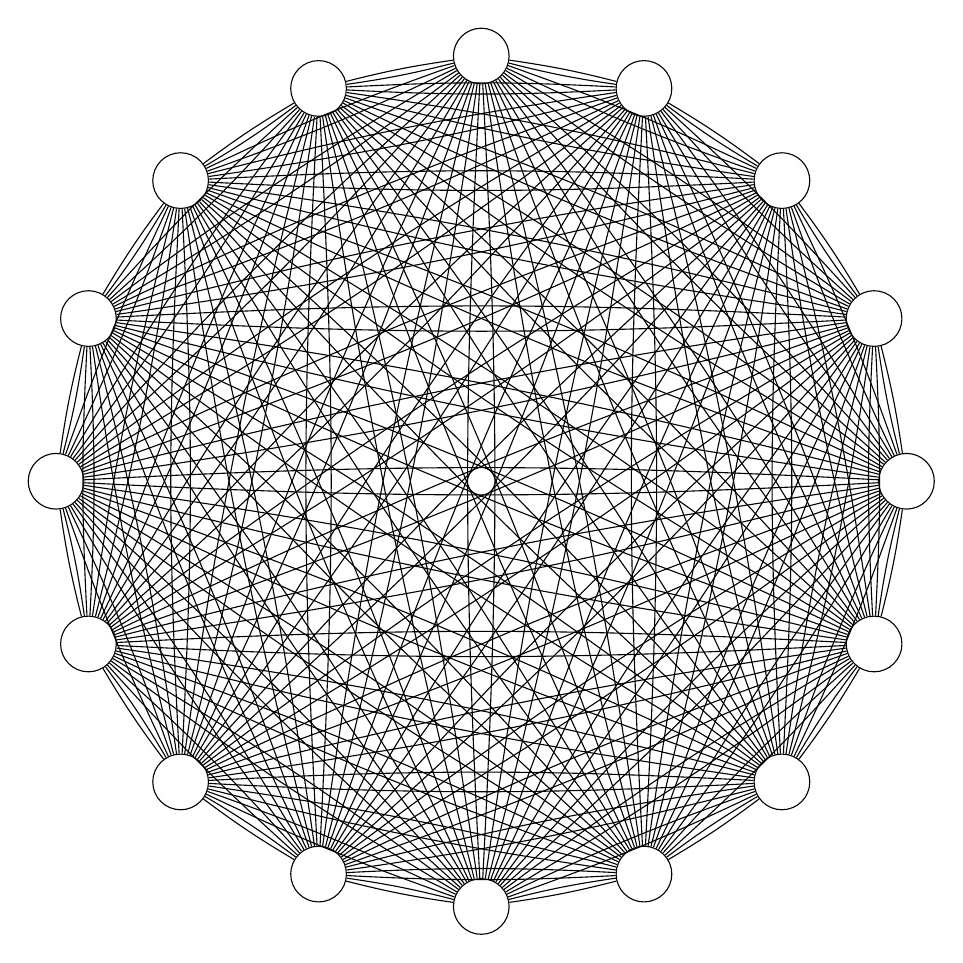
\begin{tikzpicture}[transform shape]
			\foreach \x in {1,...,16}{%
			  \pgfmathparse{(\x-1)*45+floor(\x/9)*22.5}
			  \node[draw,circle,inner sep=0.25cm] (N-\x) at (\pgfmathresult:5.4cm) {};
			} 
			\foreach \x [count=\xi from 1] in {2,...,16}{%
			  \foreach \y in {\x,...,16}{%
			  \path (N-\xi) edge[-,bend right=3] (N-\y)  edge[-,bend left=3] (N-\y);
			}
		      }
		\end{tikzpicture}
	\end{column}	
\end{columns}
\end{frame}

\begin{frame}{What is Network Density?}
	\begin{tcolorbox}[
		colback=tri_2!5!white,
		colframe=tri_2!90!black,
		title={\centering \Large $\sim$ Definition 1 --- Density $\sim$}]
		\large The tendency of a network to present direct ties between 
		pairs of nodes.
	\end{tcolorbox}
\end{frame}

\begin{frame}{Two Networks with Different Levels of Density}
	\begin{columns}[t]
		\begin{column}{0.5\textwidth}
			\begin{center}
				\textbf{A sparse network}
				\begin{figure}
					%% Creator: Matplotlib, PGF backend
%%
%% To include the figure in your LaTeX document, write
%%   \input{<filename>.pgf}
%%
%% Make sure the required packages are loaded in your preamble
%%   \usepackage{pgf}
%%
%% Also ensure that all the required font packages are loaded; for instance,
%% the lmodern package is sometimes necessary when using math font.
%%   \usepackage{lmodern}
%%
%% Figures using additional raster images can only be included by \input if
%% they are in the same directory as the main LaTeX file. For loading figures
%% from other directories you can use the `import` package
%%   \usepackage{import}
%%
%% and then include the figures with
%%   \import{<path to file>}{<filename>.pgf}
%%
%% Matplotlib used the following preamble
%%   \usepackage{fontspec}
%%   \setmainfont{DejaVuSerif.ttf}[Path=\detokenize{/Users/sbbk475/opt/anaconda3/envs/na/lib/python3.10/site-packages/matplotlib/mpl-data/fonts/ttf/}]
%%   \setsansfont{DejaVuSans.ttf}[Path=\detokenize{/Users/sbbk475/opt/anaconda3/envs/na/lib/python3.10/site-packages/matplotlib/mpl-data/fonts/ttf/}]
%%   \setmonofont{DejaVuSansMono.ttf}[Path=\detokenize{/Users/sbbk475/opt/anaconda3/envs/na/lib/python3.10/site-packages/matplotlib/mpl-data/fonts/ttf/}]
%%
\begingroup%
\makeatletter%
\begin{pgfpicture}%
\pgfpathrectangle{\pgfpointorigin}{\pgfqpoint{2.525000in}{2.510000in}}%
\pgfusepath{use as bounding box, clip}%
\begin{pgfscope}%
\pgfsetbuttcap%
\pgfsetmiterjoin%
\definecolor{currentfill}{rgb}{1.000000,1.000000,1.000000}%
\pgfsetfillcolor{currentfill}%
\pgfsetlinewidth{0.000000pt}%
\definecolor{currentstroke}{rgb}{1.000000,1.000000,1.000000}%
\pgfsetstrokecolor{currentstroke}%
\pgfsetdash{}{0pt}%
\pgfpathmoveto{\pgfqpoint{0.000000in}{0.000000in}}%
\pgfpathlineto{\pgfqpoint{2.525000in}{0.000000in}}%
\pgfpathlineto{\pgfqpoint{2.525000in}{2.510000in}}%
\pgfpathlineto{\pgfqpoint{0.000000in}{2.510000in}}%
\pgfpathlineto{\pgfqpoint{0.000000in}{0.000000in}}%
\pgfpathclose%
\pgfusepath{fill}%
\end{pgfscope}%
\begin{pgfscope}%
\pgfpathrectangle{\pgfqpoint{0.100000in}{0.100000in}}{\pgfqpoint{2.325000in}{2.310000in}}%
\pgfusepath{clip}%
\pgfsetbuttcap%
\pgfsetroundjoin%
\pgfsetlinewidth{1.003750pt}%
\definecolor{currentstroke}{rgb}{0.000000,0.000000,0.000000}%
\pgfsetstrokecolor{currentstroke}%
\pgfsetdash{}{0pt}%
\pgfpathmoveto{\pgfqpoint{0.301756in}{0.300455in}}%
\pgfpathlineto{\pgfqpoint{1.262500in}{0.300455in}}%
\pgfusepath{stroke}%
\end{pgfscope}%
\begin{pgfscope}%
\pgfpathrectangle{\pgfqpoint{0.100000in}{0.100000in}}{\pgfqpoint{2.325000in}{2.310000in}}%
\pgfusepath{clip}%
\pgfsetbuttcap%
\pgfsetroundjoin%
\pgfsetlinewidth{1.003750pt}%
\definecolor{currentstroke}{rgb}{0.000000,0.000000,0.000000}%
\pgfsetstrokecolor{currentstroke}%
\pgfsetdash{}{0pt}%
\pgfpathmoveto{\pgfqpoint{0.301756in}{0.936818in}}%
\pgfpathlineto{\pgfqpoint{1.262500in}{0.936818in}}%
\pgfusepath{stroke}%
\end{pgfscope}%
\begin{pgfscope}%
\pgfpathrectangle{\pgfqpoint{0.100000in}{0.100000in}}{\pgfqpoint{2.325000in}{2.310000in}}%
\pgfusepath{clip}%
\pgfsetbuttcap%
\pgfsetroundjoin%
\pgfsetlinewidth{1.003750pt}%
\definecolor{currentstroke}{rgb}{0.000000,0.000000,0.000000}%
\pgfsetstrokecolor{currentstroke}%
\pgfsetdash{}{0pt}%
\pgfpathmoveto{\pgfqpoint{1.262500in}{0.936818in}}%
\pgfpathlineto{\pgfqpoint{2.223244in}{0.936818in}}%
\pgfusepath{stroke}%
\end{pgfscope}%
\begin{pgfscope}%
\pgfpathrectangle{\pgfqpoint{0.100000in}{0.100000in}}{\pgfqpoint{2.325000in}{2.310000in}}%
\pgfusepath{clip}%
\pgfsetbuttcap%
\pgfsetroundjoin%
\pgfsetlinewidth{1.003750pt}%
\definecolor{currentstroke}{rgb}{0.000000,0.000000,0.000000}%
\pgfsetstrokecolor{currentstroke}%
\pgfsetdash{}{0pt}%
\pgfpathmoveto{\pgfqpoint{0.301756in}{2.209545in}}%
\pgfpathlineto{\pgfqpoint{1.262500in}{2.209545in}}%
\pgfusepath{stroke}%
\end{pgfscope}%
\begin{pgfscope}%
\pgfpathrectangle{\pgfqpoint{0.100000in}{0.100000in}}{\pgfqpoint{2.325000in}{2.310000in}}%
\pgfusepath{clip}%
\pgfsetbuttcap%
\pgfsetroundjoin%
\definecolor{currentfill}{rgb}{1.000000,1.000000,1.000000}%
\pgfsetfillcolor{currentfill}%
\pgfsetlinewidth{1.003750pt}%
\definecolor{currentstroke}{rgb}{1.000000,1.000000,1.000000}%
\pgfsetstrokecolor{currentstroke}%
\pgfsetdash{}{0pt}%
\pgfsys@defobject{currentmarker}{\pgfqpoint{-0.155282in}{-0.155282in}}{\pgfqpoint{0.155282in}{0.155282in}}{%
\pgfpathmoveto{\pgfqpoint{0.000000in}{-0.155282in}}%
\pgfpathcurveto{\pgfqpoint{0.041181in}{-0.155282in}}{\pgfqpoint{0.080682in}{-0.138921in}}{\pgfqpoint{0.109801in}{-0.109801in}}%
\pgfpathcurveto{\pgfqpoint{0.138921in}{-0.080682in}}{\pgfqpoint{0.155282in}{-0.041181in}}{\pgfqpoint{0.155282in}{0.000000in}}%
\pgfpathcurveto{\pgfqpoint{0.155282in}{0.041181in}}{\pgfqpoint{0.138921in}{0.080682in}}{\pgfqpoint{0.109801in}{0.109801in}}%
\pgfpathcurveto{\pgfqpoint{0.080682in}{0.138921in}}{\pgfqpoint{0.041181in}{0.155282in}}{\pgfqpoint{0.000000in}{0.155282in}}%
\pgfpathcurveto{\pgfqpoint{-0.041181in}{0.155282in}}{\pgfqpoint{-0.080682in}{0.138921in}}{\pgfqpoint{-0.109801in}{0.109801in}}%
\pgfpathcurveto{\pgfqpoint{-0.138921in}{0.080682in}}{\pgfqpoint{-0.155282in}{0.041181in}}{\pgfqpoint{-0.155282in}{0.000000in}}%
\pgfpathcurveto{\pgfqpoint{-0.155282in}{-0.041181in}}{\pgfqpoint{-0.138921in}{-0.080682in}}{\pgfqpoint{-0.109801in}{-0.109801in}}%
\pgfpathcurveto{\pgfqpoint{-0.080682in}{-0.138921in}}{\pgfqpoint{-0.041181in}{-0.155282in}}{\pgfqpoint{0.000000in}{-0.155282in}}%
\pgfpathlineto{\pgfqpoint{0.000000in}{-0.155282in}}%
\pgfpathclose%
\pgfusepath{stroke,fill}%
}%
\begin{pgfscope}%
\pgfsys@transformshift{0.301756in}{0.300455in}%
\pgfsys@useobject{currentmarker}{}%
\end{pgfscope}%
\begin{pgfscope}%
\pgfsys@transformshift{1.262500in}{0.300455in}%
\pgfsys@useobject{currentmarker}{}%
\end{pgfscope}%
\begin{pgfscope}%
\pgfsys@transformshift{0.301756in}{0.936818in}%
\pgfsys@useobject{currentmarker}{}%
\end{pgfscope}%
\begin{pgfscope}%
\pgfsys@transformshift{1.262500in}{0.936818in}%
\pgfsys@useobject{currentmarker}{}%
\end{pgfscope}%
\begin{pgfscope}%
\pgfsys@transformshift{2.223244in}{0.936818in}%
\pgfsys@useobject{currentmarker}{}%
\end{pgfscope}%
\begin{pgfscope}%
\pgfsys@transformshift{0.301756in}{1.573182in}%
\pgfsys@useobject{currentmarker}{}%
\end{pgfscope}%
\begin{pgfscope}%
\pgfsys@transformshift{1.262500in}{1.573182in}%
\pgfsys@useobject{currentmarker}{}%
\end{pgfscope}%
\begin{pgfscope}%
\pgfsys@transformshift{2.223244in}{1.573182in}%
\pgfsys@useobject{currentmarker}{}%
\end{pgfscope}%
\begin{pgfscope}%
\pgfsys@transformshift{0.301756in}{2.209545in}%
\pgfsys@useobject{currentmarker}{}%
\end{pgfscope}%
\begin{pgfscope}%
\pgfsys@transformshift{1.262500in}{2.209545in}%
\pgfsys@useobject{currentmarker}{}%
\end{pgfscope}%
\end{pgfscope}%
\begin{pgfscope}%
\definecolor{textcolor}{rgb}{0.000000,0.000000,0.000000}%
\pgfsetstrokecolor{textcolor}%
\pgfsetfillcolor{textcolor}%
\pgftext[x=0.301756in,y=0.300455in,,]{\color{textcolor}\sffamily\fontsize{12.000000}{14.400000}\selectfont 1}%
\end{pgfscope}%
\begin{pgfscope}%
\definecolor{textcolor}{rgb}{0.000000,0.000000,0.000000}%
\pgfsetstrokecolor{textcolor}%
\pgfsetfillcolor{textcolor}%
\pgftext[x=1.262500in,y=0.300455in,,]{\color{textcolor}\sffamily\fontsize{12.000000}{14.400000}\selectfont 2}%
\end{pgfscope}%
\begin{pgfscope}%
\definecolor{textcolor}{rgb}{0.000000,0.000000,0.000000}%
\pgfsetstrokecolor{textcolor}%
\pgfsetfillcolor{textcolor}%
\pgftext[x=0.301756in,y=0.936818in,,]{\color{textcolor}\sffamily\fontsize{12.000000}{14.400000}\selectfont 3}%
\end{pgfscope}%
\begin{pgfscope}%
\definecolor{textcolor}{rgb}{0.000000,0.000000,0.000000}%
\pgfsetstrokecolor{textcolor}%
\pgfsetfillcolor{textcolor}%
\pgftext[x=1.262500in,y=0.936818in,,]{\color{textcolor}\sffamily\fontsize{12.000000}{14.400000}\selectfont 4}%
\end{pgfscope}%
\begin{pgfscope}%
\definecolor{textcolor}{rgb}{0.000000,0.000000,0.000000}%
\pgfsetstrokecolor{textcolor}%
\pgfsetfillcolor{textcolor}%
\pgftext[x=2.223244in,y=0.936818in,,]{\color{textcolor}\sffamily\fontsize{12.000000}{14.400000}\selectfont 5}%
\end{pgfscope}%
\begin{pgfscope}%
\definecolor{textcolor}{rgb}{0.000000,0.000000,0.000000}%
\pgfsetstrokecolor{textcolor}%
\pgfsetfillcolor{textcolor}%
\pgftext[x=0.301756in,y=1.573182in,,]{\color{textcolor}\sffamily\fontsize{12.000000}{14.400000}\selectfont 6}%
\end{pgfscope}%
\begin{pgfscope}%
\definecolor{textcolor}{rgb}{0.000000,0.000000,0.000000}%
\pgfsetstrokecolor{textcolor}%
\pgfsetfillcolor{textcolor}%
\pgftext[x=1.262500in,y=1.573182in,,]{\color{textcolor}\sffamily\fontsize{12.000000}{14.400000}\selectfont 7}%
\end{pgfscope}%
\begin{pgfscope}%
\definecolor{textcolor}{rgb}{0.000000,0.000000,0.000000}%
\pgfsetstrokecolor{textcolor}%
\pgfsetfillcolor{textcolor}%
\pgftext[x=2.223244in,y=1.573182in,,]{\color{textcolor}\sffamily\fontsize{12.000000}{14.400000}\selectfont 8}%
\end{pgfscope}%
\begin{pgfscope}%
\definecolor{textcolor}{rgb}{0.000000,0.000000,0.000000}%
\pgfsetstrokecolor{textcolor}%
\pgfsetfillcolor{textcolor}%
\pgftext[x=0.301756in,y=2.209545in,,]{\color{textcolor}\sffamily\fontsize{12.000000}{14.400000}\selectfont 9}%
\end{pgfscope}%
\begin{pgfscope}%
\definecolor{textcolor}{rgb}{0.000000,0.000000,0.000000}%
\pgfsetstrokecolor{textcolor}%
\pgfsetfillcolor{textcolor}%
\pgftext[x=1.262500in,y=2.209545in,,]{\color{textcolor}\sffamily\fontsize{12.000000}{14.400000}\selectfont 10}%
\end{pgfscope}%
\end{pgfpicture}%
\makeatother%
\endgroup%

				\end{figure}
			\end{center}
		\end{column}
		\begin{column}{0.5\textwidth}
			\begin{center}
				\textbf{A dense network}
				\begin{figure}
					%% Creator: Matplotlib, PGF backend
%%
%% To include the figure in your LaTeX document, write
%%   \input{<filename>.pgf}
%%
%% Make sure the required packages are loaded in your preamble
%%   \usepackage{pgf}
%%
%% Also ensure that all the required font packages are loaded; for instance,
%% the lmodern package is sometimes necessary when using math font.
%%   \usepackage{lmodern}
%%
%% Figures using additional raster images can only be included by \input if
%% they are in the same directory as the main LaTeX file. For loading figures
%% from other directories you can use the `import` package
%%   \usepackage{import}
%%
%% and then include the figures with
%%   \import{<path to file>}{<filename>.pgf}
%%
%% Matplotlib used the following preamble
%%   \usepackage{fontspec}
%%   \setmainfont{DejaVuSerif.ttf}[Path=\detokenize{/Users/sbbk475/opt/anaconda3/envs/na/lib/python3.10/site-packages/matplotlib/mpl-data/fonts/ttf/}]
%%   \setsansfont{DejaVuSans.ttf}[Path=\detokenize{/Users/sbbk475/opt/anaconda3/envs/na/lib/python3.10/site-packages/matplotlib/mpl-data/fonts/ttf/}]
%%   \setmonofont{DejaVuSansMono.ttf}[Path=\detokenize{/Users/sbbk475/opt/anaconda3/envs/na/lib/python3.10/site-packages/matplotlib/mpl-data/fonts/ttf/}]
%%
\begingroup%
\makeatletter%
\begin{pgfpicture}%
\pgfpathrectangle{\pgfpointorigin}{\pgfqpoint{2.525000in}{2.510000in}}%
\pgfusepath{use as bounding box, clip}%
\begin{pgfscope}%
\pgfsetbuttcap%
\pgfsetmiterjoin%
\definecolor{currentfill}{rgb}{1.000000,1.000000,1.000000}%
\pgfsetfillcolor{currentfill}%
\pgfsetlinewidth{0.000000pt}%
\definecolor{currentstroke}{rgb}{1.000000,1.000000,1.000000}%
\pgfsetstrokecolor{currentstroke}%
\pgfsetdash{}{0pt}%
\pgfpathmoveto{\pgfqpoint{0.000000in}{0.000000in}}%
\pgfpathlineto{\pgfqpoint{2.525000in}{0.000000in}}%
\pgfpathlineto{\pgfqpoint{2.525000in}{2.510000in}}%
\pgfpathlineto{\pgfqpoint{0.000000in}{2.510000in}}%
\pgfpathlineto{\pgfqpoint{0.000000in}{0.000000in}}%
\pgfpathclose%
\pgfusepath{fill}%
\end{pgfscope}%
\begin{pgfscope}%
\pgfpathrectangle{\pgfqpoint{0.100000in}{0.100000in}}{\pgfqpoint{2.325000in}{2.310000in}}%
\pgfusepath{clip}%
\pgfsetbuttcap%
\pgfsetroundjoin%
\pgfsetlinewidth{1.003750pt}%
\definecolor{currentstroke}{rgb}{0.000000,0.000000,0.000000}%
\pgfsetstrokecolor{currentstroke}%
\pgfsetdash{}{0pt}%
\pgfpathmoveto{\pgfqpoint{2.223244in}{0.852927in}}%
\pgfpathlineto{\pgfqpoint{0.984016in}{1.001924in}}%
\pgfusepath{stroke}%
\end{pgfscope}%
\begin{pgfscope}%
\pgfpathrectangle{\pgfqpoint{0.100000in}{0.100000in}}{\pgfqpoint{2.325000in}{2.310000in}}%
\pgfusepath{clip}%
\pgfsetbuttcap%
\pgfsetroundjoin%
\pgfsetlinewidth{1.003750pt}%
\definecolor{currentstroke}{rgb}{0.000000,0.000000,0.000000}%
\pgfsetstrokecolor{currentstroke}%
\pgfsetdash{}{0pt}%
\pgfpathmoveto{\pgfqpoint{2.223244in}{0.852927in}}%
\pgfpathlineto{\pgfqpoint{1.404438in}{2.209545in}}%
\pgfusepath{stroke}%
\end{pgfscope}%
\begin{pgfscope}%
\pgfpathrectangle{\pgfqpoint{0.100000in}{0.100000in}}{\pgfqpoint{2.325000in}{2.310000in}}%
\pgfusepath{clip}%
\pgfsetbuttcap%
\pgfsetroundjoin%
\pgfsetlinewidth{1.003750pt}%
\definecolor{currentstroke}{rgb}{0.000000,0.000000,0.000000}%
\pgfsetstrokecolor{currentstroke}%
\pgfsetdash{}{0pt}%
\pgfpathmoveto{\pgfqpoint{2.223244in}{0.852927in}}%
\pgfpathlineto{\pgfqpoint{1.577176in}{0.331963in}}%
\pgfusepath{stroke}%
\end{pgfscope}%
\begin{pgfscope}%
\pgfpathrectangle{\pgfqpoint{0.100000in}{0.100000in}}{\pgfqpoint{2.325000in}{2.310000in}}%
\pgfusepath{clip}%
\pgfsetbuttcap%
\pgfsetroundjoin%
\pgfsetlinewidth{1.003750pt}%
\definecolor{currentstroke}{rgb}{0.000000,0.000000,0.000000}%
\pgfsetstrokecolor{currentstroke}%
\pgfsetdash{}{0pt}%
\pgfpathmoveto{\pgfqpoint{2.223244in}{0.852927in}}%
\pgfpathlineto{\pgfqpoint{2.123623in}{1.720816in}}%
\pgfusepath{stroke}%
\end{pgfscope}%
\begin{pgfscope}%
\pgfpathrectangle{\pgfqpoint{0.100000in}{0.100000in}}{\pgfqpoint{2.325000in}{2.310000in}}%
\pgfusepath{clip}%
\pgfsetbuttcap%
\pgfsetroundjoin%
\pgfsetlinewidth{1.003750pt}%
\definecolor{currentstroke}{rgb}{0.000000,0.000000,0.000000}%
\pgfsetstrokecolor{currentstroke}%
\pgfsetdash{}{0pt}%
\pgfpathmoveto{\pgfqpoint{2.223244in}{0.852927in}}%
\pgfpathlineto{\pgfqpoint{0.815031in}{0.300455in}}%
\pgfusepath{stroke}%
\end{pgfscope}%
\begin{pgfscope}%
\pgfpathrectangle{\pgfqpoint{0.100000in}{0.100000in}}{\pgfqpoint{2.325000in}{2.310000in}}%
\pgfusepath{clip}%
\pgfsetbuttcap%
\pgfsetroundjoin%
\pgfsetlinewidth{1.003750pt}%
\definecolor{currentstroke}{rgb}{0.000000,0.000000,0.000000}%
\pgfsetstrokecolor{currentstroke}%
\pgfsetdash{}{0pt}%
\pgfpathmoveto{\pgfqpoint{2.223244in}{0.852927in}}%
\pgfpathlineto{\pgfqpoint{1.672470in}{0.913328in}}%
\pgfusepath{stroke}%
\end{pgfscope}%
\begin{pgfscope}%
\pgfpathrectangle{\pgfqpoint{0.100000in}{0.100000in}}{\pgfqpoint{2.325000in}{2.310000in}}%
\pgfusepath{clip}%
\pgfsetbuttcap%
\pgfsetroundjoin%
\pgfsetlinewidth{1.003750pt}%
\definecolor{currentstroke}{rgb}{0.000000,0.000000,0.000000}%
\pgfsetstrokecolor{currentstroke}%
\pgfsetdash{}{0pt}%
\pgfpathmoveto{\pgfqpoint{0.984016in}{1.001924in}}%
\pgfpathlineto{\pgfqpoint{0.301756in}{1.155618in}}%
\pgfusepath{stroke}%
\end{pgfscope}%
\begin{pgfscope}%
\pgfpathrectangle{\pgfqpoint{0.100000in}{0.100000in}}{\pgfqpoint{2.325000in}{2.310000in}}%
\pgfusepath{clip}%
\pgfsetbuttcap%
\pgfsetroundjoin%
\pgfsetlinewidth{1.003750pt}%
\definecolor{currentstroke}{rgb}{0.000000,0.000000,0.000000}%
\pgfsetstrokecolor{currentstroke}%
\pgfsetdash{}{0pt}%
\pgfpathmoveto{\pgfqpoint{0.984016in}{1.001924in}}%
\pgfpathlineto{\pgfqpoint{0.815031in}{0.300455in}}%
\pgfusepath{stroke}%
\end{pgfscope}%
\begin{pgfscope}%
\pgfpathrectangle{\pgfqpoint{0.100000in}{0.100000in}}{\pgfqpoint{2.325000in}{2.310000in}}%
\pgfusepath{clip}%
\pgfsetbuttcap%
\pgfsetroundjoin%
\pgfsetlinewidth{1.003750pt}%
\definecolor{currentstroke}{rgb}{0.000000,0.000000,0.000000}%
\pgfsetstrokecolor{currentstroke}%
\pgfsetdash{}{0pt}%
\pgfpathmoveto{\pgfqpoint{0.984016in}{1.001924in}}%
\pgfpathlineto{\pgfqpoint{1.672470in}{0.913328in}}%
\pgfusepath{stroke}%
\end{pgfscope}%
\begin{pgfscope}%
\pgfpathrectangle{\pgfqpoint{0.100000in}{0.100000in}}{\pgfqpoint{2.325000in}{2.310000in}}%
\pgfusepath{clip}%
\pgfsetbuttcap%
\pgfsetroundjoin%
\pgfsetlinewidth{1.003750pt}%
\definecolor{currentstroke}{rgb}{0.000000,0.000000,0.000000}%
\pgfsetstrokecolor{currentstroke}%
\pgfsetdash{}{0pt}%
\pgfpathmoveto{\pgfqpoint{0.984016in}{1.001924in}}%
\pgfpathlineto{\pgfqpoint{1.404438in}{2.209545in}}%
\pgfusepath{stroke}%
\end{pgfscope}%
\begin{pgfscope}%
\pgfpathrectangle{\pgfqpoint{0.100000in}{0.100000in}}{\pgfqpoint{2.325000in}{2.310000in}}%
\pgfusepath{clip}%
\pgfsetbuttcap%
\pgfsetroundjoin%
\pgfsetlinewidth{1.003750pt}%
\definecolor{currentstroke}{rgb}{0.000000,0.000000,0.000000}%
\pgfsetstrokecolor{currentstroke}%
\pgfsetdash{}{0pt}%
\pgfpathmoveto{\pgfqpoint{0.984016in}{1.001924in}}%
\pgfpathlineto{\pgfqpoint{1.231831in}{1.667065in}}%
\pgfusepath{stroke}%
\end{pgfscope}%
\begin{pgfscope}%
\pgfpathrectangle{\pgfqpoint{0.100000in}{0.100000in}}{\pgfqpoint{2.325000in}{2.310000in}}%
\pgfusepath{clip}%
\pgfsetbuttcap%
\pgfsetroundjoin%
\pgfsetlinewidth{1.003750pt}%
\definecolor{currentstroke}{rgb}{0.000000,0.000000,0.000000}%
\pgfsetstrokecolor{currentstroke}%
\pgfsetdash{}{0pt}%
\pgfpathmoveto{\pgfqpoint{1.404438in}{2.209545in}}%
\pgfpathlineto{\pgfqpoint{0.301756in}{1.155618in}}%
\pgfusepath{stroke}%
\end{pgfscope}%
\begin{pgfscope}%
\pgfpathrectangle{\pgfqpoint{0.100000in}{0.100000in}}{\pgfqpoint{2.325000in}{2.310000in}}%
\pgfusepath{clip}%
\pgfsetbuttcap%
\pgfsetroundjoin%
\pgfsetlinewidth{1.003750pt}%
\definecolor{currentstroke}{rgb}{0.000000,0.000000,0.000000}%
\pgfsetstrokecolor{currentstroke}%
\pgfsetdash{}{0pt}%
\pgfpathmoveto{\pgfqpoint{1.404438in}{2.209545in}}%
\pgfpathlineto{\pgfqpoint{0.671251in}{1.835921in}}%
\pgfusepath{stroke}%
\end{pgfscope}%
\begin{pgfscope}%
\pgfpathrectangle{\pgfqpoint{0.100000in}{0.100000in}}{\pgfqpoint{2.325000in}{2.310000in}}%
\pgfusepath{clip}%
\pgfsetbuttcap%
\pgfsetroundjoin%
\pgfsetlinewidth{1.003750pt}%
\definecolor{currentstroke}{rgb}{0.000000,0.000000,0.000000}%
\pgfsetstrokecolor{currentstroke}%
\pgfsetdash{}{0pt}%
\pgfpathmoveto{\pgfqpoint{1.404438in}{2.209545in}}%
\pgfpathlineto{\pgfqpoint{2.123623in}{1.720816in}}%
\pgfusepath{stroke}%
\end{pgfscope}%
\begin{pgfscope}%
\pgfpathrectangle{\pgfqpoint{0.100000in}{0.100000in}}{\pgfqpoint{2.325000in}{2.310000in}}%
\pgfusepath{clip}%
\pgfsetbuttcap%
\pgfsetroundjoin%
\pgfsetlinewidth{1.003750pt}%
\definecolor{currentstroke}{rgb}{0.000000,0.000000,0.000000}%
\pgfsetstrokecolor{currentstroke}%
\pgfsetdash{}{0pt}%
\pgfpathmoveto{\pgfqpoint{1.404438in}{2.209545in}}%
\pgfpathlineto{\pgfqpoint{1.231831in}{1.667065in}}%
\pgfusepath{stroke}%
\end{pgfscope}%
\begin{pgfscope}%
\pgfpathrectangle{\pgfqpoint{0.100000in}{0.100000in}}{\pgfqpoint{2.325000in}{2.310000in}}%
\pgfusepath{clip}%
\pgfsetbuttcap%
\pgfsetroundjoin%
\pgfsetlinewidth{1.003750pt}%
\definecolor{currentstroke}{rgb}{0.000000,0.000000,0.000000}%
\pgfsetstrokecolor{currentstroke}%
\pgfsetdash{}{0pt}%
\pgfpathmoveto{\pgfqpoint{0.301756in}{1.155618in}}%
\pgfpathlineto{\pgfqpoint{0.671251in}{1.835921in}}%
\pgfusepath{stroke}%
\end{pgfscope}%
\begin{pgfscope}%
\pgfpathrectangle{\pgfqpoint{0.100000in}{0.100000in}}{\pgfqpoint{2.325000in}{2.310000in}}%
\pgfusepath{clip}%
\pgfsetbuttcap%
\pgfsetroundjoin%
\pgfsetlinewidth{1.003750pt}%
\definecolor{currentstroke}{rgb}{0.000000,0.000000,0.000000}%
\pgfsetstrokecolor{currentstroke}%
\pgfsetdash{}{0pt}%
\pgfpathmoveto{\pgfqpoint{0.301756in}{1.155618in}}%
\pgfpathlineto{\pgfqpoint{1.577176in}{0.331963in}}%
\pgfusepath{stroke}%
\end{pgfscope}%
\begin{pgfscope}%
\pgfpathrectangle{\pgfqpoint{0.100000in}{0.100000in}}{\pgfqpoint{2.325000in}{2.310000in}}%
\pgfusepath{clip}%
\pgfsetbuttcap%
\pgfsetroundjoin%
\pgfsetlinewidth{1.003750pt}%
\definecolor{currentstroke}{rgb}{0.000000,0.000000,0.000000}%
\pgfsetstrokecolor{currentstroke}%
\pgfsetdash{}{0pt}%
\pgfpathmoveto{\pgfqpoint{0.301756in}{1.155618in}}%
\pgfpathlineto{\pgfqpoint{1.231831in}{1.667065in}}%
\pgfusepath{stroke}%
\end{pgfscope}%
\begin{pgfscope}%
\pgfpathrectangle{\pgfqpoint{0.100000in}{0.100000in}}{\pgfqpoint{2.325000in}{2.310000in}}%
\pgfusepath{clip}%
\pgfsetbuttcap%
\pgfsetroundjoin%
\pgfsetlinewidth{1.003750pt}%
\definecolor{currentstroke}{rgb}{0.000000,0.000000,0.000000}%
\pgfsetstrokecolor{currentstroke}%
\pgfsetdash{}{0pt}%
\pgfpathmoveto{\pgfqpoint{0.301756in}{1.155618in}}%
\pgfpathlineto{\pgfqpoint{0.815031in}{0.300455in}}%
\pgfusepath{stroke}%
\end{pgfscope}%
\begin{pgfscope}%
\pgfpathrectangle{\pgfqpoint{0.100000in}{0.100000in}}{\pgfqpoint{2.325000in}{2.310000in}}%
\pgfusepath{clip}%
\pgfsetbuttcap%
\pgfsetroundjoin%
\pgfsetlinewidth{1.003750pt}%
\definecolor{currentstroke}{rgb}{0.000000,0.000000,0.000000}%
\pgfsetstrokecolor{currentstroke}%
\pgfsetdash{}{0pt}%
\pgfpathmoveto{\pgfqpoint{1.672470in}{0.913328in}}%
\pgfpathlineto{\pgfqpoint{0.671251in}{1.835921in}}%
\pgfusepath{stroke}%
\end{pgfscope}%
\begin{pgfscope}%
\pgfpathrectangle{\pgfqpoint{0.100000in}{0.100000in}}{\pgfqpoint{2.325000in}{2.310000in}}%
\pgfusepath{clip}%
\pgfsetbuttcap%
\pgfsetroundjoin%
\pgfsetlinewidth{1.003750pt}%
\definecolor{currentstroke}{rgb}{0.000000,0.000000,0.000000}%
\pgfsetstrokecolor{currentstroke}%
\pgfsetdash{}{0pt}%
\pgfpathmoveto{\pgfqpoint{1.672470in}{0.913328in}}%
\pgfpathlineto{\pgfqpoint{0.815031in}{0.300455in}}%
\pgfusepath{stroke}%
\end{pgfscope}%
\begin{pgfscope}%
\pgfpathrectangle{\pgfqpoint{0.100000in}{0.100000in}}{\pgfqpoint{2.325000in}{2.310000in}}%
\pgfusepath{clip}%
\pgfsetbuttcap%
\pgfsetroundjoin%
\pgfsetlinewidth{1.003750pt}%
\definecolor{currentstroke}{rgb}{0.000000,0.000000,0.000000}%
\pgfsetstrokecolor{currentstroke}%
\pgfsetdash{}{0pt}%
\pgfpathmoveto{\pgfqpoint{1.672470in}{0.913328in}}%
\pgfpathlineto{\pgfqpoint{1.577176in}{0.331963in}}%
\pgfusepath{stroke}%
\end{pgfscope}%
\begin{pgfscope}%
\pgfpathrectangle{\pgfqpoint{0.100000in}{0.100000in}}{\pgfqpoint{2.325000in}{2.310000in}}%
\pgfusepath{clip}%
\pgfsetbuttcap%
\pgfsetroundjoin%
\pgfsetlinewidth{1.003750pt}%
\definecolor{currentstroke}{rgb}{0.000000,0.000000,0.000000}%
\pgfsetstrokecolor{currentstroke}%
\pgfsetdash{}{0pt}%
\pgfpathmoveto{\pgfqpoint{1.672470in}{0.913328in}}%
\pgfpathlineto{\pgfqpoint{2.123623in}{1.720816in}}%
\pgfusepath{stroke}%
\end{pgfscope}%
\begin{pgfscope}%
\pgfpathrectangle{\pgfqpoint{0.100000in}{0.100000in}}{\pgfqpoint{2.325000in}{2.310000in}}%
\pgfusepath{clip}%
\pgfsetbuttcap%
\pgfsetroundjoin%
\pgfsetlinewidth{1.003750pt}%
\definecolor{currentstroke}{rgb}{0.000000,0.000000,0.000000}%
\pgfsetstrokecolor{currentstroke}%
\pgfsetdash{}{0pt}%
\pgfpathmoveto{\pgfqpoint{0.671251in}{1.835921in}}%
\pgfpathlineto{\pgfqpoint{0.815031in}{0.300455in}}%
\pgfusepath{stroke}%
\end{pgfscope}%
\begin{pgfscope}%
\pgfpathrectangle{\pgfqpoint{0.100000in}{0.100000in}}{\pgfqpoint{2.325000in}{2.310000in}}%
\pgfusepath{clip}%
\pgfsetbuttcap%
\pgfsetroundjoin%
\pgfsetlinewidth{1.003750pt}%
\definecolor{currentstroke}{rgb}{0.000000,0.000000,0.000000}%
\pgfsetstrokecolor{currentstroke}%
\pgfsetdash{}{0pt}%
\pgfpathmoveto{\pgfqpoint{0.671251in}{1.835921in}}%
\pgfpathlineto{\pgfqpoint{1.231831in}{1.667065in}}%
\pgfusepath{stroke}%
\end{pgfscope}%
\begin{pgfscope}%
\pgfpathrectangle{\pgfqpoint{0.100000in}{0.100000in}}{\pgfqpoint{2.325000in}{2.310000in}}%
\pgfusepath{clip}%
\pgfsetbuttcap%
\pgfsetroundjoin%
\pgfsetlinewidth{1.003750pt}%
\definecolor{currentstroke}{rgb}{0.000000,0.000000,0.000000}%
\pgfsetstrokecolor{currentstroke}%
\pgfsetdash{}{0pt}%
\pgfpathmoveto{\pgfqpoint{0.671251in}{1.835921in}}%
\pgfpathlineto{\pgfqpoint{2.123623in}{1.720816in}}%
\pgfusepath{stroke}%
\end{pgfscope}%
\begin{pgfscope}%
\pgfpathrectangle{\pgfqpoint{0.100000in}{0.100000in}}{\pgfqpoint{2.325000in}{2.310000in}}%
\pgfusepath{clip}%
\pgfsetbuttcap%
\pgfsetroundjoin%
\pgfsetlinewidth{1.003750pt}%
\definecolor{currentstroke}{rgb}{0.000000,0.000000,0.000000}%
\pgfsetstrokecolor{currentstroke}%
\pgfsetdash{}{0pt}%
\pgfpathmoveto{\pgfqpoint{0.815031in}{0.300455in}}%
\pgfpathlineto{\pgfqpoint{1.577176in}{0.331963in}}%
\pgfusepath{stroke}%
\end{pgfscope}%
\begin{pgfscope}%
\pgfpathrectangle{\pgfqpoint{0.100000in}{0.100000in}}{\pgfqpoint{2.325000in}{2.310000in}}%
\pgfusepath{clip}%
\pgfsetbuttcap%
\pgfsetroundjoin%
\pgfsetlinewidth{1.003750pt}%
\definecolor{currentstroke}{rgb}{0.000000,0.000000,0.000000}%
\pgfsetstrokecolor{currentstroke}%
\pgfsetdash{}{0pt}%
\pgfpathmoveto{\pgfqpoint{1.577176in}{0.331963in}}%
\pgfpathlineto{\pgfqpoint{1.231831in}{1.667065in}}%
\pgfusepath{stroke}%
\end{pgfscope}%
\begin{pgfscope}%
\pgfpathrectangle{\pgfqpoint{0.100000in}{0.100000in}}{\pgfqpoint{2.325000in}{2.310000in}}%
\pgfusepath{clip}%
\pgfsetbuttcap%
\pgfsetroundjoin%
\pgfsetlinewidth{1.003750pt}%
\definecolor{currentstroke}{rgb}{0.000000,0.000000,0.000000}%
\pgfsetstrokecolor{currentstroke}%
\pgfsetdash{}{0pt}%
\pgfpathmoveto{\pgfqpoint{1.577176in}{0.331963in}}%
\pgfpathlineto{\pgfqpoint{2.123623in}{1.720816in}}%
\pgfusepath{stroke}%
\end{pgfscope}%
\begin{pgfscope}%
\pgfpathrectangle{\pgfqpoint{0.100000in}{0.100000in}}{\pgfqpoint{2.325000in}{2.310000in}}%
\pgfusepath{clip}%
\pgfsetbuttcap%
\pgfsetroundjoin%
\pgfsetlinewidth{1.003750pt}%
\definecolor{currentstroke}{rgb}{0.000000,0.000000,0.000000}%
\pgfsetstrokecolor{currentstroke}%
\pgfsetdash{}{0pt}%
\pgfpathmoveto{\pgfqpoint{1.231831in}{1.667065in}}%
\pgfpathlineto{\pgfqpoint{2.123623in}{1.720816in}}%
\pgfusepath{stroke}%
\end{pgfscope}%
\begin{pgfscope}%
\pgfpathrectangle{\pgfqpoint{0.100000in}{0.100000in}}{\pgfqpoint{2.325000in}{2.310000in}}%
\pgfusepath{clip}%
\pgfsetbuttcap%
\pgfsetroundjoin%
\definecolor{currentfill}{rgb}{1.000000,1.000000,1.000000}%
\pgfsetfillcolor{currentfill}%
\pgfsetlinewidth{1.003750pt}%
\definecolor{currentstroke}{rgb}{1.000000,1.000000,1.000000}%
\pgfsetstrokecolor{currentstroke}%
\pgfsetdash{}{0pt}%
\pgfsys@defobject{currentmarker}{\pgfqpoint{-0.155282in}{-0.155282in}}{\pgfqpoint{0.155282in}{0.155282in}}{%
\pgfpathmoveto{\pgfqpoint{0.000000in}{-0.155282in}}%
\pgfpathcurveto{\pgfqpoint{0.041181in}{-0.155282in}}{\pgfqpoint{0.080682in}{-0.138921in}}{\pgfqpoint{0.109801in}{-0.109801in}}%
\pgfpathcurveto{\pgfqpoint{0.138921in}{-0.080682in}}{\pgfqpoint{0.155282in}{-0.041181in}}{\pgfqpoint{0.155282in}{0.000000in}}%
\pgfpathcurveto{\pgfqpoint{0.155282in}{0.041181in}}{\pgfqpoint{0.138921in}{0.080682in}}{\pgfqpoint{0.109801in}{0.109801in}}%
\pgfpathcurveto{\pgfqpoint{0.080682in}{0.138921in}}{\pgfqpoint{0.041181in}{0.155282in}}{\pgfqpoint{0.000000in}{0.155282in}}%
\pgfpathcurveto{\pgfqpoint{-0.041181in}{0.155282in}}{\pgfqpoint{-0.080682in}{0.138921in}}{\pgfqpoint{-0.109801in}{0.109801in}}%
\pgfpathcurveto{\pgfqpoint{-0.138921in}{0.080682in}}{\pgfqpoint{-0.155282in}{0.041181in}}{\pgfqpoint{-0.155282in}{0.000000in}}%
\pgfpathcurveto{\pgfqpoint{-0.155282in}{-0.041181in}}{\pgfqpoint{-0.138921in}{-0.080682in}}{\pgfqpoint{-0.109801in}{-0.109801in}}%
\pgfpathcurveto{\pgfqpoint{-0.080682in}{-0.138921in}}{\pgfqpoint{-0.041181in}{-0.155282in}}{\pgfqpoint{0.000000in}{-0.155282in}}%
\pgfpathlineto{\pgfqpoint{0.000000in}{-0.155282in}}%
\pgfpathclose%
\pgfusepath{stroke,fill}%
}%
\begin{pgfscope}%
\pgfsys@transformshift{2.223244in}{0.852927in}%
\pgfsys@useobject{currentmarker}{}%
\end{pgfscope}%
\begin{pgfscope}%
\pgfsys@transformshift{0.984016in}{1.001924in}%
\pgfsys@useobject{currentmarker}{}%
\end{pgfscope}%
\begin{pgfscope}%
\pgfsys@transformshift{1.404438in}{2.209545in}%
\pgfsys@useobject{currentmarker}{}%
\end{pgfscope}%
\begin{pgfscope}%
\pgfsys@transformshift{0.301756in}{1.155618in}%
\pgfsys@useobject{currentmarker}{}%
\end{pgfscope}%
\begin{pgfscope}%
\pgfsys@transformshift{1.672470in}{0.913328in}%
\pgfsys@useobject{currentmarker}{}%
\end{pgfscope}%
\begin{pgfscope}%
\pgfsys@transformshift{0.671251in}{1.835921in}%
\pgfsys@useobject{currentmarker}{}%
\end{pgfscope}%
\begin{pgfscope}%
\pgfsys@transformshift{0.815031in}{0.300455in}%
\pgfsys@useobject{currentmarker}{}%
\end{pgfscope}%
\begin{pgfscope}%
\pgfsys@transformshift{1.577176in}{0.331963in}%
\pgfsys@useobject{currentmarker}{}%
\end{pgfscope}%
\begin{pgfscope}%
\pgfsys@transformshift{1.231831in}{1.667065in}%
\pgfsys@useobject{currentmarker}{}%
\end{pgfscope}%
\begin{pgfscope}%
\pgfsys@transformshift{2.123623in}{1.720816in}%
\pgfsys@useobject{currentmarker}{}%
\end{pgfscope}%
\end{pgfscope}%
\begin{pgfscope}%
\definecolor{textcolor}{rgb}{0.000000,0.000000,0.000000}%
\pgfsetstrokecolor{textcolor}%
\pgfsetfillcolor{textcolor}%
\pgftext[x=2.223244in,y=0.852927in,,]{\color{textcolor}\sffamily\fontsize{12.000000}{14.400000}\selectfont 3}%
\end{pgfscope}%
\begin{pgfscope}%
\definecolor{textcolor}{rgb}{0.000000,0.000000,0.000000}%
\pgfsetstrokecolor{textcolor}%
\pgfsetfillcolor{textcolor}%
\pgftext[x=0.984016in,y=1.001924in,,]{\color{textcolor}\sffamily\fontsize{12.000000}{14.400000}\selectfont 4}%
\end{pgfscope}%
\begin{pgfscope}%
\definecolor{textcolor}{rgb}{0.000000,0.000000,0.000000}%
\pgfsetstrokecolor{textcolor}%
\pgfsetfillcolor{textcolor}%
\pgftext[x=1.404438in,y=2.209545in,,]{\color{textcolor}\sffamily\fontsize{12.000000}{14.400000}\selectfont 7}%
\end{pgfscope}%
\begin{pgfscope}%
\definecolor{textcolor}{rgb}{0.000000,0.000000,0.000000}%
\pgfsetstrokecolor{textcolor}%
\pgfsetfillcolor{textcolor}%
\pgftext[x=0.301756in,y=1.155618in,,]{\color{textcolor}\sffamily\fontsize{12.000000}{14.400000}\selectfont 5}%
\end{pgfscope}%
\begin{pgfscope}%
\definecolor{textcolor}{rgb}{0.000000,0.000000,0.000000}%
\pgfsetstrokecolor{textcolor}%
\pgfsetfillcolor{textcolor}%
\pgftext[x=1.672470in,y=0.913328in,,]{\color{textcolor}\sffamily\fontsize{12.000000}{14.400000}\selectfont 0}%
\end{pgfscope}%
\begin{pgfscope}%
\definecolor{textcolor}{rgb}{0.000000,0.000000,0.000000}%
\pgfsetstrokecolor{textcolor}%
\pgfsetfillcolor{textcolor}%
\pgftext[x=0.671251in,y=1.835921in,,]{\color{textcolor}\sffamily\fontsize{12.000000}{14.400000}\selectfont 2}%
\end{pgfscope}%
\begin{pgfscope}%
\definecolor{textcolor}{rgb}{0.000000,0.000000,0.000000}%
\pgfsetstrokecolor{textcolor}%
\pgfsetfillcolor{textcolor}%
\pgftext[x=0.815031in,y=0.300455in,,]{\color{textcolor}\sffamily\fontsize{12.000000}{14.400000}\selectfont 8}%
\end{pgfscope}%
\begin{pgfscope}%
\definecolor{textcolor}{rgb}{0.000000,0.000000,0.000000}%
\pgfsetstrokecolor{textcolor}%
\pgfsetfillcolor{textcolor}%
\pgftext[x=1.577176in,y=0.331963in,,]{\color{textcolor}\sffamily\fontsize{12.000000}{14.400000}\selectfont 9}%
\end{pgfscope}%
\begin{pgfscope}%
\definecolor{textcolor}{rgb}{0.000000,0.000000,0.000000}%
\pgfsetstrokecolor{textcolor}%
\pgfsetfillcolor{textcolor}%
\pgftext[x=1.231831in,y=1.667065in,,]{\color{textcolor}\sffamily\fontsize{12.000000}{14.400000}\selectfont 1}%
\end{pgfscope}%
\begin{pgfscope}%
\definecolor{textcolor}{rgb}{0.000000,0.000000,0.000000}%
\pgfsetstrokecolor{textcolor}%
\pgfsetfillcolor{textcolor}%
\pgftext[x=2.123623in,y=1.720816in,,]{\color{textcolor}\sffamily\fontsize{12.000000}{14.400000}\selectfont 6}%
\end{pgfscope}%
\end{pgfpicture}%
\makeatother%
\endgroup%

				\end{figure}
			\end{center}
		\end{column}
	\end{columns}
\end{frame}

\begin{frame}{What Is the Outcome of Dense Networks?}
	\begin{figure}
		\resizebox{0.85\textwidth}{!}{
		\begin{tikzpicture}[node distance=1cm, auto,] % no additional information
		\node[](d){};
		\node[punkt,left=2cm of d](dn){Network density};
		\node[punkt, label={[align=right]}, right=2cm of d](bsc){Bonding\\social capital}
		edge[pil, <-, bend left=0](dn.east);
		\node[above=0.15cm of d](edge_label){\textcolor{blue}{\textit{fosters}}};
		\node[below=0.15cm of d](d0){};
		\node[right=3.35cm of d0](d1){};
                \node[right=0.001cm of d1](d2){};
		\node[right=0.001cm of d2](d3){};
		\node[below=-0.2cm of dn](d5){};
                \node[right=0.001cm of d5](d4){};
		\node[left=0.001cm of d5](d6){};
		\pause
		\node[punkt, below=0.65cm of d](info_sharing){Information sharing}
		edge[pil, <-, bend left=30](d4)
		edge[pil, ->, bend right=30] (d1.south);
		\pause 
		\node[below=-0.2cm of info_sharing](info_sharing_1){}
		edge[pil, ->](cooperation.north);
		\pause
		\node[punkt, below=0.65cm of info_sharing](cooperation){Cooperation}
		edge[pil, <-, bend left=30](d5)
		edge[pil, ->, bend right=30] (d2.south);
		\pause
		\node[below=-0.2cm of cooperation](cooperation_1){}
		edge[pil, ->](trust.north);
		\pause
		\node[punkt, below=0.65cm of cooperation](trust){Trust}
		edge[pil, <-, bend left=30](d6)
		edge[pil, ->, bend right=30] (d3.south);
		% \node[left=3cm of novelty](d1){};
		% %edge[pil, bend left=20](novelty.north);
		% \node[punkt,blue, below=1.5cm of d1](structure){Social structure of collaboration}
		% edge[pil, bend right=20](novelty.south);
		% \node[punkt,blue,below=5cm of d1](employment){Employment relationships---HR}
		% edge[pil,blue,<-, bend left=50](structure.west);
		% %edge[pil, bend right=50](structure.east);
		% \node[left=5cm of d1](d2){};
		% \node[punkb, below=2cm of d2](mobility){};
		% %edge[pil, bend right=0](novelty.west)
		% %edge[pil, <-, bend right=45](employment.west)
		% %edge[pil, <-, bend left=40](valuation.west)
		% %edge[pil, bend left=60](structure.north);
		% %\node[left=2cm of mobility](d3){};
		% \node[punkb, above=1.5cm of d2](jolts){};
		% %edge[pil, bend left=0](valuation.west);
		\end{tikzpicture}}
	\end{figure}
\end{frame}

\begin{frame}
	{Network Density $\rightarrow$ Information Sharing}
	{A pricing problem: setup}
	\begin{small}
	Let us consider the following pricing problem:
	\begin{itemize}
		\item The potential transaction includes a buyer $B$ and a 
		seller $S$ 
		\item The market is not regulated and there is no perfect 
		information on the vector of prices in the market
		\item $S$ already produced the good and sustained a unitary 
		production cost $\delta$
		\item We take the perspective of $S$, which `makes the price' 
		based on the best available information on the reservation 
		price of $B$ and competitors'
		offering prices $\Phi = \{\phi_{1}, \phi{_2}, ..., \phi_{i},
		..., \phi_{N}\}$
		\item The pay-off of $S$ is as follows:
	\end{itemize}
	\[
		\Pi^{S}=
		\begin{dcases}
			\hat\phi - \delta & \text{if B willing to buy}\\
			-\delta                            & \text{otherwise}\\
		\end{dcases}
	\]
	\begin{itemize}
		\item 
		The probability $B$ is willing to buy is expressed as
	\end{itemize}	

		\begin{equation*}
			p = f(\phi) \text{\quad \quad with \quad } 0 \leq  p \leq 1 
		\end{equation*}
	\end{small}
\end{frame}

\begin{frame}
	{Network Density $\rightarrow$ Information Sharing}
	{A pricing problem: the expected pay-off}
	Per the previous slide, the expected pay-off for $S$ is

	\begin{equation*}
		E(\Pi^{S}) = p * (\phi - \delta) + (1 - p) * (- \delta)
	\end{equation*}

	\begin{figure}
		\begin{center}
			%% Creator: Matplotlib, PGF backend
%%
%% To include the figure in your LaTeX document, write
%%   \input{<filename>.pgf}
%%
%% Make sure the required packages are loaded in your preamble
%%   \usepackage{pgf}
%%
%% Also ensure that all the required font packages are loaded; for instance,
%% the lmodern package is sometimes necessary when using math font.
%%   \usepackage{lmodern}
%%
%% Figures using additional raster images can only be included by \input if
%% they are in the same directory as the main LaTeX file. For loading figures
%% from other directories you can use the `import` package
%%   \usepackage{import}
%%
%% and then include the figures with
%%   \import{<path to file>}{<filename>.pgf}
%%
%% Matplotlib used the following preamble
%%   \usepackage{fontspec}
%%   \setmainfont{DejaVuSerif.ttf}[Path=\detokenize{/Users/sbbk475/opt/anaconda3/envs/na/lib/python3.10/site-packages/matplotlib/mpl-data/fonts/ttf/}]
%%   \setsansfont{DejaVuSans.ttf}[Path=\detokenize{/Users/sbbk475/opt/anaconda3/envs/na/lib/python3.10/site-packages/matplotlib/mpl-data/fonts/ttf/}]
%%   \setmonofont{DejaVuSansMono.ttf}[Path=\detokenize{/Users/sbbk475/opt/anaconda3/envs/na/lib/python3.10/site-packages/matplotlib/mpl-data/fonts/ttf/}]
%%
\begingroup%
\makeatletter%
\begin{pgfpicture}%
\pgfpathrectangle{\pgfpointorigin}{\pgfqpoint{2.933101in}{2.556079in}}%
\pgfusepath{use as bounding box, clip}%
\begin{pgfscope}%
\pgfsetbuttcap%
\pgfsetmiterjoin%
\definecolor{currentfill}{rgb}{1.000000,1.000000,1.000000}%
\pgfsetfillcolor{currentfill}%
\pgfsetlinewidth{0.000000pt}%
\definecolor{currentstroke}{rgb}{1.000000,1.000000,1.000000}%
\pgfsetstrokecolor{currentstroke}%
\pgfsetdash{}{0pt}%
\pgfpathmoveto{\pgfqpoint{0.000000in}{0.000000in}}%
\pgfpathlineto{\pgfqpoint{2.933101in}{0.000000in}}%
\pgfpathlineto{\pgfqpoint{2.933101in}{2.556079in}}%
\pgfpathlineto{\pgfqpoint{0.000000in}{2.556079in}}%
\pgfpathlineto{\pgfqpoint{0.000000in}{0.000000in}}%
\pgfpathclose%
\pgfusepath{fill}%
\end{pgfscope}%
\begin{pgfscope}%
\pgfsetbuttcap%
\pgfsetmiterjoin%
\definecolor{currentfill}{rgb}{1.000000,1.000000,1.000000}%
\pgfsetfillcolor{currentfill}%
\pgfsetlinewidth{0.000000pt}%
\definecolor{currentstroke}{rgb}{0.000000,0.000000,0.000000}%
\pgfsetstrokecolor{currentstroke}%
\pgfsetstrokeopacity{0.000000}%
\pgfsetdash{}{0pt}%
\pgfpathmoveto{\pgfqpoint{0.343056in}{0.338579in}}%
\pgfpathlineto{\pgfqpoint{2.474306in}{0.338579in}}%
\pgfpathlineto{\pgfqpoint{2.474306in}{2.456079in}}%
\pgfpathlineto{\pgfqpoint{0.343056in}{2.456079in}}%
\pgfpathlineto{\pgfqpoint{0.343056in}{0.338579in}}%
\pgfpathclose%
\pgfusepath{fill}%
\end{pgfscope}%
\begin{pgfscope}%
\definecolor{textcolor}{rgb}{0.000000,0.000000,0.000000}%
\pgfsetstrokecolor{textcolor}%
\pgfsetfillcolor{textcolor}%
\pgftext[x=1.408681in,y=0.234413in,,top]{\color{textcolor}\sffamily\fontsize{10.000000}{12.000000}\selectfont \(\displaystyle \phi\)}%
\end{pgfscope}%
\begin{pgfscope}%
\definecolor{textcolor}{rgb}{0.000000,0.000000,0.000000}%
\pgfsetstrokecolor{textcolor}%
\pgfsetfillcolor{textcolor}%
\pgftext[x=0.238889in,y=1.397329in,,bottom,rotate=90.000000]{\color{textcolor}\sffamily\fontsize{10.000000}{12.000000}\selectfont \(\displaystyle E(\Pi)\)}%
\end{pgfscope}%
\begin{pgfscope}%
\pgfpathrectangle{\pgfqpoint{0.343056in}{0.338579in}}{\pgfqpoint{2.131250in}{2.117500in}}%
\pgfusepath{clip}%
\pgfsetrectcap%
\pgfsetroundjoin%
\pgfsetlinewidth{1.505625pt}%
\definecolor{currentstroke}{rgb}{0.000000,0.000000,0.000000}%
\pgfsetstrokecolor{currentstroke}%
\pgfsetdash{}{0pt}%
\pgfpathmoveto{\pgfqpoint{0.439931in}{0.434829in}}%
\pgfpathlineto{\pgfqpoint{0.459501in}{0.511829in}}%
\pgfpathlineto{\pgfqpoint{0.479072in}{0.587258in}}%
\pgfpathlineto{\pgfqpoint{0.498643in}{0.661115in}}%
\pgfpathlineto{\pgfqpoint{0.518213in}{0.733401in}}%
\pgfpathlineto{\pgfqpoint{0.537784in}{0.804115in}}%
\pgfpathlineto{\pgfqpoint{0.557355in}{0.873258in}}%
\pgfpathlineto{\pgfqpoint{0.576926in}{0.940829in}}%
\pgfpathlineto{\pgfqpoint{0.596496in}{1.006829in}}%
\pgfpathlineto{\pgfqpoint{0.616067in}{1.071258in}}%
\pgfpathlineto{\pgfqpoint{0.635638in}{1.134115in}}%
\pgfpathlineto{\pgfqpoint{0.655208in}{1.195401in}}%
\pgfpathlineto{\pgfqpoint{0.674779in}{1.255115in}}%
\pgfpathlineto{\pgfqpoint{0.694350in}{1.313258in}}%
\pgfpathlineto{\pgfqpoint{0.713920in}{1.369829in}}%
\pgfpathlineto{\pgfqpoint{0.733491in}{1.424829in}}%
\pgfpathlineto{\pgfqpoint{0.753062in}{1.478258in}}%
\pgfpathlineto{\pgfqpoint{0.772633in}{1.530115in}}%
\pgfpathlineto{\pgfqpoint{0.792203in}{1.580401in}}%
\pgfpathlineto{\pgfqpoint{0.811774in}{1.629115in}}%
\pgfpathlineto{\pgfqpoint{0.831345in}{1.676258in}}%
\pgfpathlineto{\pgfqpoint{0.850915in}{1.721829in}}%
\pgfpathlineto{\pgfqpoint{0.870486in}{1.765829in}}%
\pgfpathlineto{\pgfqpoint{0.890057in}{1.808258in}}%
\pgfpathlineto{\pgfqpoint{0.909628in}{1.849115in}}%
\pgfpathlineto{\pgfqpoint{0.929198in}{1.888401in}}%
\pgfpathlineto{\pgfqpoint{0.948769in}{1.926115in}}%
\pgfpathlineto{\pgfqpoint{0.968340in}{1.962258in}}%
\pgfpathlineto{\pgfqpoint{0.987910in}{1.996829in}}%
\pgfpathlineto{\pgfqpoint{1.007481in}{2.029829in}}%
\pgfpathlineto{\pgfqpoint{1.027052in}{2.061258in}}%
\pgfpathlineto{\pgfqpoint{1.046622in}{2.091115in}}%
\pgfpathlineto{\pgfqpoint{1.066193in}{2.119401in}}%
\pgfpathlineto{\pgfqpoint{1.085764in}{2.146115in}}%
\pgfpathlineto{\pgfqpoint{1.105335in}{2.171258in}}%
\pgfpathlineto{\pgfqpoint{1.124905in}{2.194829in}}%
\pgfpathlineto{\pgfqpoint{1.144476in}{2.216829in}}%
\pgfpathlineto{\pgfqpoint{1.164047in}{2.237258in}}%
\pgfpathlineto{\pgfqpoint{1.183617in}{2.256115in}}%
\pgfpathlineto{\pgfqpoint{1.203188in}{2.273401in}}%
\pgfpathlineto{\pgfqpoint{1.222759in}{2.289115in}}%
\pgfpathlineto{\pgfqpoint{1.242330in}{2.303258in}}%
\pgfpathlineto{\pgfqpoint{1.261900in}{2.315829in}}%
\pgfpathlineto{\pgfqpoint{1.281471in}{2.326829in}}%
\pgfpathlineto{\pgfqpoint{1.301042in}{2.336258in}}%
\pgfpathlineto{\pgfqpoint{1.320612in}{2.344115in}}%
\pgfpathlineto{\pgfqpoint{1.340183in}{2.350401in}}%
\pgfpathlineto{\pgfqpoint{1.359754in}{2.355115in}}%
\pgfpathlineto{\pgfqpoint{1.379324in}{2.358258in}}%
\pgfpathlineto{\pgfqpoint{1.398895in}{2.359829in}}%
\pgfpathlineto{\pgfqpoint{1.418466in}{2.359829in}}%
\pgfpathlineto{\pgfqpoint{1.438037in}{2.358258in}}%
\pgfpathlineto{\pgfqpoint{1.457607in}{2.355115in}}%
\pgfpathlineto{\pgfqpoint{1.477178in}{2.350401in}}%
\pgfpathlineto{\pgfqpoint{1.496749in}{2.344115in}}%
\pgfpathlineto{\pgfqpoint{1.516319in}{2.336258in}}%
\pgfpathlineto{\pgfqpoint{1.535890in}{2.326829in}}%
\pgfpathlineto{\pgfqpoint{1.555461in}{2.315829in}}%
\pgfpathlineto{\pgfqpoint{1.575032in}{2.303258in}}%
\pgfpathlineto{\pgfqpoint{1.594602in}{2.289115in}}%
\pgfpathlineto{\pgfqpoint{1.614173in}{2.273401in}}%
\pgfpathlineto{\pgfqpoint{1.633744in}{2.256115in}}%
\pgfpathlineto{\pgfqpoint{1.653314in}{2.237258in}}%
\pgfpathlineto{\pgfqpoint{1.672885in}{2.216829in}}%
\pgfpathlineto{\pgfqpoint{1.692456in}{2.194829in}}%
\pgfpathlineto{\pgfqpoint{1.712027in}{2.171258in}}%
\pgfpathlineto{\pgfqpoint{1.731597in}{2.146115in}}%
\pgfpathlineto{\pgfqpoint{1.751168in}{2.119401in}}%
\pgfpathlineto{\pgfqpoint{1.770739in}{2.091115in}}%
\pgfpathlineto{\pgfqpoint{1.790309in}{2.061258in}}%
\pgfpathlineto{\pgfqpoint{1.809880in}{2.029829in}}%
\pgfpathlineto{\pgfqpoint{1.829451in}{1.996829in}}%
\pgfpathlineto{\pgfqpoint{1.849021in}{1.962258in}}%
\pgfpathlineto{\pgfqpoint{1.868592in}{1.926115in}}%
\pgfpathlineto{\pgfqpoint{1.888163in}{1.888401in}}%
\pgfpathlineto{\pgfqpoint{1.907734in}{1.849115in}}%
\pgfpathlineto{\pgfqpoint{1.927304in}{1.808258in}}%
\pgfpathlineto{\pgfqpoint{1.946875in}{1.765829in}}%
\pgfpathlineto{\pgfqpoint{1.966446in}{1.721829in}}%
\pgfpathlineto{\pgfqpoint{1.986016in}{1.676258in}}%
\pgfpathlineto{\pgfqpoint{2.005587in}{1.629115in}}%
\pgfpathlineto{\pgfqpoint{2.025158in}{1.580401in}}%
\pgfpathlineto{\pgfqpoint{2.044729in}{1.530115in}}%
\pgfpathlineto{\pgfqpoint{2.064299in}{1.478258in}}%
\pgfpathlineto{\pgfqpoint{2.083870in}{1.424829in}}%
\pgfpathlineto{\pgfqpoint{2.103441in}{1.369829in}}%
\pgfpathlineto{\pgfqpoint{2.123011in}{1.313258in}}%
\pgfpathlineto{\pgfqpoint{2.142582in}{1.255115in}}%
\pgfpathlineto{\pgfqpoint{2.162153in}{1.195401in}}%
\pgfpathlineto{\pgfqpoint{2.181723in}{1.134115in}}%
\pgfpathlineto{\pgfqpoint{2.201294in}{1.071258in}}%
\pgfpathlineto{\pgfqpoint{2.220865in}{1.006829in}}%
\pgfpathlineto{\pgfqpoint{2.240436in}{0.940829in}}%
\pgfpathlineto{\pgfqpoint{2.260006in}{0.873258in}}%
\pgfpathlineto{\pgfqpoint{2.279577in}{0.804115in}}%
\pgfpathlineto{\pgfqpoint{2.299148in}{0.733401in}}%
\pgfpathlineto{\pgfqpoint{2.318718in}{0.661115in}}%
\pgfpathlineto{\pgfqpoint{2.338289in}{0.587258in}}%
\pgfpathlineto{\pgfqpoint{2.357860in}{0.511829in}}%
\pgfpathlineto{\pgfqpoint{2.377431in}{0.434829in}}%
\pgfusepath{stroke}%
\end{pgfscope}%
\begin{pgfscope}%
\pgfpathrectangle{\pgfqpoint{0.343056in}{0.338579in}}{\pgfqpoint{2.131250in}{2.117500in}}%
\pgfusepath{clip}%
\pgfsetbuttcap%
\pgfsetroundjoin%
\pgfsetlinewidth{1.505625pt}%
\definecolor{currentstroke}{rgb}{0.501961,0.501961,0.501961}%
\pgfsetstrokecolor{currentstroke}%
\pgfsetdash{{5.550000pt}{2.400000pt}}{0.000000pt}%
\pgfpathmoveto{\pgfqpoint{0.439931in}{1.589947in}}%
\pgfpathlineto{\pgfqpoint{2.377431in}{1.589947in}}%
\pgfusepath{stroke}%
\end{pgfscope}%
\begin{pgfscope}%
\pgfpathrectangle{\pgfqpoint{0.343056in}{0.338579in}}{\pgfqpoint{2.131250in}{2.117500in}}%
\pgfusepath{clip}%
\pgfsetbuttcap%
\pgfsetroundjoin%
\pgfsetlinewidth{1.505625pt}%
\definecolor{currentstroke}{rgb}{1.000000,0.000000,0.000000}%
\pgfsetstrokecolor{currentstroke}%
\pgfsetdash{{5.550000pt}{2.400000pt}}{0.000000pt}%
\pgfpathmoveto{\pgfqpoint{0.439931in}{0.434829in}}%
\pgfpathlineto{\pgfqpoint{2.377431in}{0.434829in}}%
\pgfusepath{stroke}%
\end{pgfscope}%
\begin{pgfscope}%
\definecolor{textcolor}{rgb}{0.000000,0.000000,0.000000}%
\pgfsetstrokecolor{textcolor}%
\pgfsetfillcolor{textcolor}%
\pgftext[x=2.474306in,y=1.551443in,left,base]{\color{textcolor}\sffamily\fontsize{10.000000}{12.000000}\selectfont \(\displaystyle \Pi = 0\)}%
\end{pgfscope}%
\begin{pgfscope}%
\definecolor{textcolor}{rgb}{0.000000,0.000000,0.000000}%
\pgfsetstrokecolor{textcolor}%
\pgfsetfillcolor{textcolor}%
\pgftext[x=0.149306in,y=0.396326in,left,base]{\color{textcolor}\sffamily\fontsize{10.000000}{12.000000}\selectfont \(\displaystyle -\delta\)}%
\end{pgfscope}%
\end{pgfpicture}%
\makeatother%
\endgroup%

		\end{center}
	\end{figure}
	
\end{frame}

\begin{frame}
	{Network Density $\rightarrow$ Information Sharing}
	{What is the fair market price? Scenario A: sparse network}
	\centering
	\begin{columns}
		\begin{column}{0.5\textwidth}
			%% Creator: Matplotlib, PGF backend
%%
%% To include the figure in your LaTeX document, write
%%   \input{<filename>.pgf}
%%
%% Make sure the required packages are loaded in your preamble
%%   \usepackage{pgf}
%%
%% Also ensure that all the required font packages are loaded; for instance,
%% the lmodern package is sometimes necessary when using math font.
%%   \usepackage{lmodern}
%%
%% Figures using additional raster images can only be included by \input if
%% they are in the same directory as the main LaTeX file. For loading figures
%% from other directories you can use the `import` package
%%   \usepackage{import}
%%
%% and then include the figures with
%%   \import{<path to file>}{<filename>.pgf}
%%
%% Matplotlib used the following preamble
%%   \usepackage{fontspec}
%%   \setmainfont{DejaVuSerif.ttf}[Path=\detokenize{/Users/sbbk475/opt/anaconda3/envs/na/lib/python3.10/site-packages/matplotlib/mpl-data/fonts/ttf/}]
%%   \setsansfont{DejaVuSans.ttf}[Path=\detokenize{/Users/sbbk475/opt/anaconda3/envs/na/lib/python3.10/site-packages/matplotlib/mpl-data/fonts/ttf/}]
%%   \setmonofont{DejaVuSansMono.ttf}[Path=\detokenize{/Users/sbbk475/opt/anaconda3/envs/na/lib/python3.10/site-packages/matplotlib/mpl-data/fonts/ttf/}]
%%
\begingroup%
\makeatletter%
\begin{pgfpicture}%
\pgfpathrectangle{\pgfpointorigin}{\pgfqpoint{2.933101in}{2.556079in}}%
\pgfusepath{use as bounding box, clip}%
\begin{pgfscope}%
\pgfsetbuttcap%
\pgfsetmiterjoin%
\definecolor{currentfill}{rgb}{1.000000,1.000000,1.000000}%
\pgfsetfillcolor{currentfill}%
\pgfsetlinewidth{0.000000pt}%
\definecolor{currentstroke}{rgb}{1.000000,1.000000,1.000000}%
\pgfsetstrokecolor{currentstroke}%
\pgfsetdash{}{0pt}%
\pgfpathmoveto{\pgfqpoint{0.000000in}{0.000000in}}%
\pgfpathlineto{\pgfqpoint{2.933101in}{0.000000in}}%
\pgfpathlineto{\pgfqpoint{2.933101in}{2.556079in}}%
\pgfpathlineto{\pgfqpoint{0.000000in}{2.556079in}}%
\pgfpathlineto{\pgfqpoint{0.000000in}{0.000000in}}%
\pgfpathclose%
\pgfusepath{fill}%
\end{pgfscope}%
\begin{pgfscope}%
\pgfsetbuttcap%
\pgfsetmiterjoin%
\definecolor{currentfill}{rgb}{1.000000,1.000000,1.000000}%
\pgfsetfillcolor{currentfill}%
\pgfsetlinewidth{0.000000pt}%
\definecolor{currentstroke}{rgb}{0.000000,0.000000,0.000000}%
\pgfsetstrokecolor{currentstroke}%
\pgfsetstrokeopacity{0.000000}%
\pgfsetdash{}{0pt}%
\pgfpathmoveto{\pgfqpoint{0.343056in}{0.338579in}}%
\pgfpathlineto{\pgfqpoint{2.474306in}{0.338579in}}%
\pgfpathlineto{\pgfqpoint{2.474306in}{2.456079in}}%
\pgfpathlineto{\pgfqpoint{0.343056in}{2.456079in}}%
\pgfpathlineto{\pgfqpoint{0.343056in}{0.338579in}}%
\pgfpathclose%
\pgfusepath{fill}%
\end{pgfscope}%
\begin{pgfscope}%
\definecolor{textcolor}{rgb}{0.000000,0.000000,0.000000}%
\pgfsetstrokecolor{textcolor}%
\pgfsetfillcolor{textcolor}%
\pgftext[x=1.408681in,y=0.234413in,,top]{\color{textcolor}\sffamily\fontsize{10.000000}{12.000000}\selectfont \(\displaystyle \phi\)}%
\end{pgfscope}%
\begin{pgfscope}%
\definecolor{textcolor}{rgb}{0.000000,0.000000,0.000000}%
\pgfsetstrokecolor{textcolor}%
\pgfsetfillcolor{textcolor}%
\pgftext[x=0.238889in,y=1.397329in,,bottom,rotate=90.000000]{\color{textcolor}\sffamily\fontsize{10.000000}{12.000000}\selectfont \(\displaystyle E(\Pi)\)}%
\end{pgfscope}%
\begin{pgfscope}%
\pgfpathrectangle{\pgfqpoint{0.343056in}{0.338579in}}{\pgfqpoint{2.131250in}{2.117500in}}%
\pgfusepath{clip}%
\pgfsetrectcap%
\pgfsetroundjoin%
\pgfsetlinewidth{1.505625pt}%
\definecolor{currentstroke}{rgb}{0.000000,0.000000,0.000000}%
\pgfsetstrokecolor{currentstroke}%
\pgfsetdash{}{0pt}%
\pgfpathmoveto{\pgfqpoint{0.439931in}{0.434829in}}%
\pgfpathlineto{\pgfqpoint{0.459501in}{0.511829in}}%
\pgfpathlineto{\pgfqpoint{0.479072in}{0.587258in}}%
\pgfpathlineto{\pgfqpoint{0.498643in}{0.661115in}}%
\pgfpathlineto{\pgfqpoint{0.518213in}{0.733401in}}%
\pgfpathlineto{\pgfqpoint{0.537784in}{0.804115in}}%
\pgfpathlineto{\pgfqpoint{0.557355in}{0.873258in}}%
\pgfpathlineto{\pgfqpoint{0.576926in}{0.940829in}}%
\pgfpathlineto{\pgfqpoint{0.596496in}{1.006829in}}%
\pgfpathlineto{\pgfqpoint{0.616067in}{1.071258in}}%
\pgfpathlineto{\pgfqpoint{0.635638in}{1.134115in}}%
\pgfpathlineto{\pgfqpoint{0.655208in}{1.195401in}}%
\pgfpathlineto{\pgfqpoint{0.674779in}{1.255115in}}%
\pgfpathlineto{\pgfqpoint{0.694350in}{1.313258in}}%
\pgfpathlineto{\pgfqpoint{0.713920in}{1.369829in}}%
\pgfpathlineto{\pgfqpoint{0.733491in}{1.424829in}}%
\pgfpathlineto{\pgfqpoint{0.753062in}{1.478258in}}%
\pgfpathlineto{\pgfqpoint{0.772633in}{1.530115in}}%
\pgfpathlineto{\pgfqpoint{0.792203in}{1.580401in}}%
\pgfpathlineto{\pgfqpoint{0.811774in}{1.629115in}}%
\pgfpathlineto{\pgfqpoint{0.831345in}{1.676258in}}%
\pgfpathlineto{\pgfqpoint{0.850915in}{1.721829in}}%
\pgfpathlineto{\pgfqpoint{0.870486in}{1.765829in}}%
\pgfpathlineto{\pgfqpoint{0.890057in}{1.808258in}}%
\pgfpathlineto{\pgfqpoint{0.909628in}{1.849115in}}%
\pgfpathlineto{\pgfqpoint{0.929198in}{1.888401in}}%
\pgfpathlineto{\pgfqpoint{0.948769in}{1.926115in}}%
\pgfpathlineto{\pgfqpoint{0.968340in}{1.962258in}}%
\pgfpathlineto{\pgfqpoint{0.987910in}{1.996829in}}%
\pgfpathlineto{\pgfqpoint{1.007481in}{2.029829in}}%
\pgfpathlineto{\pgfqpoint{1.027052in}{2.061258in}}%
\pgfpathlineto{\pgfqpoint{1.046622in}{2.091115in}}%
\pgfpathlineto{\pgfqpoint{1.066193in}{2.119401in}}%
\pgfpathlineto{\pgfqpoint{1.085764in}{2.146115in}}%
\pgfpathlineto{\pgfqpoint{1.105335in}{2.171258in}}%
\pgfpathlineto{\pgfqpoint{1.124905in}{2.194829in}}%
\pgfpathlineto{\pgfqpoint{1.144476in}{2.216829in}}%
\pgfpathlineto{\pgfqpoint{1.164047in}{2.237258in}}%
\pgfpathlineto{\pgfqpoint{1.183617in}{2.256115in}}%
\pgfpathlineto{\pgfqpoint{1.203188in}{2.273401in}}%
\pgfpathlineto{\pgfqpoint{1.222759in}{2.289115in}}%
\pgfpathlineto{\pgfqpoint{1.242330in}{2.303258in}}%
\pgfpathlineto{\pgfqpoint{1.261900in}{2.315829in}}%
\pgfpathlineto{\pgfqpoint{1.281471in}{2.326829in}}%
\pgfpathlineto{\pgfqpoint{1.301042in}{2.336258in}}%
\pgfpathlineto{\pgfqpoint{1.320612in}{2.344115in}}%
\pgfpathlineto{\pgfqpoint{1.340183in}{2.350401in}}%
\pgfpathlineto{\pgfqpoint{1.359754in}{2.355115in}}%
\pgfpathlineto{\pgfqpoint{1.379324in}{2.358258in}}%
\pgfpathlineto{\pgfqpoint{1.398895in}{2.359829in}}%
\pgfpathlineto{\pgfqpoint{1.418466in}{2.359829in}}%
\pgfpathlineto{\pgfqpoint{1.438037in}{2.358258in}}%
\pgfpathlineto{\pgfqpoint{1.457607in}{2.355115in}}%
\pgfpathlineto{\pgfqpoint{1.477178in}{2.350401in}}%
\pgfpathlineto{\pgfqpoint{1.496749in}{2.344115in}}%
\pgfpathlineto{\pgfqpoint{1.516319in}{2.336258in}}%
\pgfpathlineto{\pgfqpoint{1.535890in}{2.326829in}}%
\pgfpathlineto{\pgfqpoint{1.555461in}{2.315829in}}%
\pgfpathlineto{\pgfqpoint{1.575032in}{2.303258in}}%
\pgfpathlineto{\pgfqpoint{1.594602in}{2.289115in}}%
\pgfpathlineto{\pgfqpoint{1.614173in}{2.273401in}}%
\pgfpathlineto{\pgfqpoint{1.633744in}{2.256115in}}%
\pgfpathlineto{\pgfqpoint{1.653314in}{2.237258in}}%
\pgfpathlineto{\pgfqpoint{1.672885in}{2.216829in}}%
\pgfpathlineto{\pgfqpoint{1.692456in}{2.194829in}}%
\pgfpathlineto{\pgfqpoint{1.712027in}{2.171258in}}%
\pgfpathlineto{\pgfqpoint{1.731597in}{2.146115in}}%
\pgfpathlineto{\pgfqpoint{1.751168in}{2.119401in}}%
\pgfpathlineto{\pgfqpoint{1.770739in}{2.091115in}}%
\pgfpathlineto{\pgfqpoint{1.790309in}{2.061258in}}%
\pgfpathlineto{\pgfqpoint{1.809880in}{2.029829in}}%
\pgfpathlineto{\pgfqpoint{1.829451in}{1.996829in}}%
\pgfpathlineto{\pgfqpoint{1.849021in}{1.962258in}}%
\pgfpathlineto{\pgfqpoint{1.868592in}{1.926115in}}%
\pgfpathlineto{\pgfqpoint{1.888163in}{1.888401in}}%
\pgfpathlineto{\pgfqpoint{1.907734in}{1.849115in}}%
\pgfpathlineto{\pgfqpoint{1.927304in}{1.808258in}}%
\pgfpathlineto{\pgfqpoint{1.946875in}{1.765829in}}%
\pgfpathlineto{\pgfqpoint{1.966446in}{1.721829in}}%
\pgfpathlineto{\pgfqpoint{1.986016in}{1.676258in}}%
\pgfpathlineto{\pgfqpoint{2.005587in}{1.629115in}}%
\pgfpathlineto{\pgfqpoint{2.025158in}{1.580401in}}%
\pgfpathlineto{\pgfqpoint{2.044729in}{1.530115in}}%
\pgfpathlineto{\pgfqpoint{2.064299in}{1.478258in}}%
\pgfpathlineto{\pgfqpoint{2.083870in}{1.424829in}}%
\pgfpathlineto{\pgfqpoint{2.103441in}{1.369829in}}%
\pgfpathlineto{\pgfqpoint{2.123011in}{1.313258in}}%
\pgfpathlineto{\pgfqpoint{2.142582in}{1.255115in}}%
\pgfpathlineto{\pgfqpoint{2.162153in}{1.195401in}}%
\pgfpathlineto{\pgfqpoint{2.181723in}{1.134115in}}%
\pgfpathlineto{\pgfqpoint{2.201294in}{1.071258in}}%
\pgfpathlineto{\pgfqpoint{2.220865in}{1.006829in}}%
\pgfpathlineto{\pgfqpoint{2.240436in}{0.940829in}}%
\pgfpathlineto{\pgfqpoint{2.260006in}{0.873258in}}%
\pgfpathlineto{\pgfqpoint{2.279577in}{0.804115in}}%
\pgfpathlineto{\pgfqpoint{2.299148in}{0.733401in}}%
\pgfpathlineto{\pgfqpoint{2.318718in}{0.661115in}}%
\pgfpathlineto{\pgfqpoint{2.338289in}{0.587258in}}%
\pgfpathlineto{\pgfqpoint{2.357860in}{0.511829in}}%
\pgfpathlineto{\pgfqpoint{2.377431in}{0.434829in}}%
\pgfusepath{stroke}%
\end{pgfscope}%
\begin{pgfscope}%
\pgfpathrectangle{\pgfqpoint{0.343056in}{0.338579in}}{\pgfqpoint{2.131250in}{2.117500in}}%
\pgfusepath{clip}%
\pgfsetbuttcap%
\pgfsetroundjoin%
\pgfsetlinewidth{1.505625pt}%
\definecolor{currentstroke}{rgb}{0.501961,0.501961,0.501961}%
\pgfsetstrokecolor{currentstroke}%
\pgfsetdash{{5.550000pt}{2.400000pt}}{0.000000pt}%
\pgfpathmoveto{\pgfqpoint{0.439931in}{1.589947in}}%
\pgfpathlineto{\pgfqpoint{2.377431in}{1.589947in}}%
\pgfusepath{stroke}%
\end{pgfscope}%
\begin{pgfscope}%
\pgfpathrectangle{\pgfqpoint{0.343056in}{0.338579in}}{\pgfqpoint{2.131250in}{2.117500in}}%
\pgfusepath{clip}%
\pgfsetbuttcap%
\pgfsetroundjoin%
\pgfsetlinewidth{1.505625pt}%
\definecolor{currentstroke}{rgb}{1.000000,0.000000,0.000000}%
\pgfsetstrokecolor{currentstroke}%
\pgfsetdash{{5.550000pt}{2.400000pt}}{0.000000pt}%
\pgfpathmoveto{\pgfqpoint{0.439931in}{0.434829in}}%
\pgfpathlineto{\pgfqpoint{2.377431in}{0.434829in}}%
\pgfusepath{stroke}%
\end{pgfscope}%
\begin{pgfscope}%
\definecolor{textcolor}{rgb}{0.000000,0.000000,0.000000}%
\pgfsetstrokecolor{textcolor}%
\pgfsetfillcolor{textcolor}%
\pgftext[x=2.474306in,y=1.551443in,left,base]{\color{textcolor}\sffamily\fontsize{10.000000}{12.000000}\selectfont \(\displaystyle \Pi = 0\)}%
\end{pgfscope}%
\begin{pgfscope}%
\definecolor{textcolor}{rgb}{0.000000,0.000000,0.000000}%
\pgfsetstrokecolor{textcolor}%
\pgfsetfillcolor{textcolor}%
\pgftext[x=0.149306in,y=0.396326in,left,base]{\color{textcolor}\sffamily\fontsize{10.000000}{12.000000}\selectfont \(\displaystyle -\delta\)}%
\end{pgfscope}%
\end{pgfpicture}%
\makeatother%
\endgroup%

		\end{column}
		\begin{column}{0.5\textwidth}
			%% Creator: Matplotlib, PGF backend
%%
%% To include the figure in your LaTeX document, write
%%   \input{<filename>.pgf}
%%
%% Make sure the required packages are loaded in your preamble
%%   \usepackage{pgf}
%%
%% Also ensure that all the required font packages are loaded; for instance,
%% the lmodern package is sometimes necessary when using math font.
%%   \usepackage{lmodern}
%%
%% Figures using additional raster images can only be included by \input if
%% they are in the same directory as the main LaTeX file. For loading figures
%% from other directories you can use the `import` package
%%   \usepackage{import}
%%
%% and then include the figures with
%%   \import{<path to file>}{<filename>.pgf}
%%
%% Matplotlib used the following preamble
%%   \usepackage{fontspec}
%%   \setmainfont{DejaVuSerif.ttf}[Path=\detokenize{/Users/sbbk475/opt/anaconda3/envs/na/lib/python3.10/site-packages/matplotlib/mpl-data/fonts/ttf/}]
%%   \setsansfont{DejaVuSans.ttf}[Path=\detokenize{/Users/sbbk475/opt/anaconda3/envs/na/lib/python3.10/site-packages/matplotlib/mpl-data/fonts/ttf/}]
%%   \setmonofont{DejaVuSansMono.ttf}[Path=\detokenize{/Users/sbbk475/opt/anaconda3/envs/na/lib/python3.10/site-packages/matplotlib/mpl-data/fonts/ttf/}]
%%
\begingroup%
\makeatletter%
\begin{pgfpicture}%
\pgfpathrectangle{\pgfpointorigin}{\pgfqpoint{2.677079in}{2.114497in}}%
\pgfusepath{use as bounding box, clip}%
\begin{pgfscope}%
\pgfsetbuttcap%
\pgfsetmiterjoin%
\definecolor{currentfill}{rgb}{1.000000,1.000000,1.000000}%
\pgfsetfillcolor{currentfill}%
\pgfsetlinewidth{0.000000pt}%
\definecolor{currentstroke}{rgb}{1.000000,1.000000,1.000000}%
\pgfsetstrokecolor{currentstroke}%
\pgfsetdash{}{0pt}%
\pgfpathmoveto{\pgfqpoint{0.000000in}{0.000000in}}%
\pgfpathlineto{\pgfqpoint{2.677079in}{0.000000in}}%
\pgfpathlineto{\pgfqpoint{2.677079in}{2.114497in}}%
\pgfpathlineto{\pgfqpoint{0.000000in}{2.114497in}}%
\pgfpathlineto{\pgfqpoint{0.000000in}{0.000000in}}%
\pgfpathclose%
\pgfusepath{fill}%
\end{pgfscope}%
\begin{pgfscope}%
\pgfpathrectangle{\pgfqpoint{0.252079in}{0.100000in}}{\pgfqpoint{2.325000in}{1.540000in}}%
\pgfusepath{clip}%
\pgfsetbuttcap%
\pgfsetroundjoin%
\pgfsetlinewidth{1.003750pt}%
\definecolor{currentstroke}{rgb}{0.000000,0.000000,0.000000}%
\pgfsetstrokecolor{currentstroke}%
\pgfsetdash{}{0pt}%
\pgfpathmoveto{\pgfqpoint{1.904324in}{0.852927in}}%
\pgfpathlineto{\pgfqpoint{1.388803in}{1.535854in}}%
\pgfusepath{stroke}%
\end{pgfscope}%
\begin{pgfscope}%
\pgfpathrectangle{\pgfqpoint{0.252079in}{0.100000in}}{\pgfqpoint{2.325000in}{1.540000in}}%
\pgfusepath{clip}%
\pgfsetbuttcap%
\pgfsetroundjoin%
\pgfsetlinewidth{1.003750pt}%
\definecolor{currentstroke}{rgb}{0.000000,0.000000,0.000000}%
\pgfsetstrokecolor{currentstroke}%
\pgfsetdash{}{0pt}%
\pgfpathmoveto{\pgfqpoint{1.904324in}{0.852927in}}%
\pgfpathlineto{\pgfqpoint{2.419845in}{1.535854in}}%
\pgfusepath{stroke}%
\end{pgfscope}%
\begin{pgfscope}%
\pgfpathrectangle{\pgfqpoint{0.252079in}{0.100000in}}{\pgfqpoint{2.325000in}{1.540000in}}%
\pgfusepath{clip}%
\pgfsetbuttcap%
\pgfsetroundjoin%
\definecolor{currentfill}{rgb}{1.000000,1.000000,1.000000}%
\pgfsetfillcolor{currentfill}%
\pgfsetlinewidth{1.003750pt}%
\definecolor{currentstroke}{rgb}{1.000000,1.000000,1.000000}%
\pgfsetstrokecolor{currentstroke}%
\pgfsetdash{}{0pt}%
\pgfsys@defobject{currentmarker}{\pgfqpoint{-0.120281in}{-0.120281in}}{\pgfqpoint{0.120281in}{0.120281in}}{%
\pgfpathmoveto{\pgfqpoint{0.000000in}{-0.120281in}}%
\pgfpathcurveto{\pgfqpoint{0.031899in}{-0.120281in}}{\pgfqpoint{0.062496in}{-0.107608in}}{\pgfqpoint{0.085052in}{-0.085052in}}%
\pgfpathcurveto{\pgfqpoint{0.107608in}{-0.062496in}}{\pgfqpoint{0.120281in}{-0.031899in}}{\pgfqpoint{0.120281in}{0.000000in}}%
\pgfpathcurveto{\pgfqpoint{0.120281in}{0.031899in}}{\pgfqpoint{0.107608in}{0.062496in}}{\pgfqpoint{0.085052in}{0.085052in}}%
\pgfpathcurveto{\pgfqpoint{0.062496in}{0.107608in}}{\pgfqpoint{0.031899in}{0.120281in}}{\pgfqpoint{0.000000in}{0.120281in}}%
\pgfpathcurveto{\pgfqpoint{-0.031899in}{0.120281in}}{\pgfqpoint{-0.062496in}{0.107608in}}{\pgfqpoint{-0.085052in}{0.085052in}}%
\pgfpathcurveto{\pgfqpoint{-0.107608in}{0.062496in}}{\pgfqpoint{-0.120281in}{0.031899in}}{\pgfqpoint{-0.120281in}{0.000000in}}%
\pgfpathcurveto{\pgfqpoint{-0.120281in}{-0.031899in}}{\pgfqpoint{-0.107608in}{-0.062496in}}{\pgfqpoint{-0.085052in}{-0.085052in}}%
\pgfpathcurveto{\pgfqpoint{-0.062496in}{-0.107608in}}{\pgfqpoint{-0.031899in}{-0.120281in}}{\pgfqpoint{0.000000in}{-0.120281in}}%
\pgfpathlineto{\pgfqpoint{0.000000in}{-0.120281in}}%
\pgfpathclose%
\pgfusepath{stroke,fill}%
}%
\begin{pgfscope}%
\pgfsys@transformshift{0.357761in}{0.170000in}%
\pgfsys@useobject{currentmarker}{}%
\end{pgfscope}%
\begin{pgfscope}%
\pgfsys@transformshift{0.357761in}{0.852927in}%
\pgfsys@useobject{currentmarker}{}%
\end{pgfscope}%
\begin{pgfscope}%
\pgfsys@transformshift{0.357761in}{1.535854in}%
\pgfsys@useobject{currentmarker}{}%
\end{pgfscope}%
\begin{pgfscope}%
\pgfsys@transformshift{1.904324in}{0.852927in}%
\pgfsys@useobject{currentmarker}{}%
\end{pgfscope}%
\begin{pgfscope}%
\pgfsys@transformshift{1.388803in}{1.535854in}%
\pgfsys@useobject{currentmarker}{}%
\end{pgfscope}%
\begin{pgfscope}%
\pgfsys@transformshift{2.419845in}{1.535854in}%
\pgfsys@useobject{currentmarker}{}%
\end{pgfscope}%
\begin{pgfscope}%
\pgfsys@transformshift{1.904324in}{0.170000in}%
\pgfsys@useobject{currentmarker}{}%
\end{pgfscope}%
\end{pgfscope}%
\begin{pgfscope}%
\definecolor{textcolor}{rgb}{0.000000,0.000000,0.000000}%
\pgfsetstrokecolor{textcolor}%
\pgfsetfillcolor{textcolor}%
\pgftext[x=0.357761in,y=0.170000in,,]{\color{textcolor}\sffamily\fontsize{12.000000}{14.400000}\selectfont b1}%
\end{pgfscope}%
\begin{pgfscope}%
\definecolor{textcolor}{rgb}{0.000000,0.000000,0.000000}%
\pgfsetstrokecolor{textcolor}%
\pgfsetfillcolor{textcolor}%
\pgftext[x=0.357761in,y=0.852927in,,]{\color{textcolor}\sffamily\fontsize{12.000000}{14.400000}\selectfont b2}%
\end{pgfscope}%
\begin{pgfscope}%
\definecolor{textcolor}{rgb}{0.000000,0.000000,0.000000}%
\pgfsetstrokecolor{textcolor}%
\pgfsetfillcolor{textcolor}%
\pgftext[x=0.357761in,y=1.535854in,,]{\color{textcolor}\sffamily\fontsize{12.000000}{14.400000}\selectfont b3}%
\end{pgfscope}%
\begin{pgfscope}%
\definecolor{textcolor}{rgb}{0.000000,0.000000,0.000000}%
\pgfsetstrokecolor{textcolor}%
\pgfsetfillcolor{textcolor}%
\pgftext[x=1.904324in,y=0.852927in,,]{\color{textcolor}\sffamily\fontsize{12.000000}{14.400000}\selectfont s1}%
\end{pgfscope}%
\begin{pgfscope}%
\definecolor{textcolor}{rgb}{0.000000,0.000000,0.000000}%
\pgfsetstrokecolor{textcolor}%
\pgfsetfillcolor{textcolor}%
\pgftext[x=1.388803in,y=1.535854in,,]{\color{textcolor}\sffamily\fontsize{12.000000}{14.400000}\selectfont s2}%
\end{pgfscope}%
\begin{pgfscope}%
\definecolor{textcolor}{rgb}{0.000000,0.000000,0.000000}%
\pgfsetstrokecolor{textcolor}%
\pgfsetfillcolor{textcolor}%
\pgftext[x=2.419845in,y=1.535854in,,]{\color{textcolor}\sffamily\fontsize{12.000000}{14.400000}\selectfont s3}%
\end{pgfscope}%
\begin{pgfscope}%
\definecolor{textcolor}{rgb}{0.000000,0.000000,0.000000}%
\pgfsetstrokecolor{textcolor}%
\pgfsetfillcolor{textcolor}%
\pgftext[x=1.904324in,y=0.170000in,,]{\color{textcolor}\sffamily\fontsize{12.000000}{14.400000}\selectfont s4}%
\end{pgfscope}%
\begin{pgfscope}%
\definecolor{textcolor}{rgb}{0.000000,0.000000,0.000000}%
\pgfsetstrokecolor{textcolor}%
\pgfsetfillcolor{textcolor}%
\pgftext[x=0.100000in,y=1.877317in,left,base]{\color{textcolor}\sffamily\fontsize{13.000000}{15.600000}\selectfont Buyers}%
\end{pgfscope}%
\begin{pgfscope}%
\definecolor{textcolor}{rgb}{0.000000,0.000000,0.000000}%
\pgfsetstrokecolor{textcolor}%
\pgfsetfillcolor{textcolor}%
\pgftext[x=1.646563in,y=1.877317in,left,base]{\color{textcolor}\sffamily\fontsize{13.000000}{15.600000}\selectfont Sellers}%
\end{pgfscope}%
\end{pgfpicture}%
\makeatother%
\endgroup%

		\end{column}
	\end{columns}
\end{frame}

\begin{frame}
	{Network Density $\rightarrow$ Information Sharing}
	{What is the fair market price? Scenario A: sparse network}
	\centering
	\begin{columns}
		\begin{column}{0.5\textwidth}
			%% Creator: Matplotlib, PGF backend
%%
%% To include the figure in your LaTeX document, write
%%   \input{<filename>.pgf}
%%
%% Make sure the required packages are loaded in your preamble
%%   \usepackage{pgf}
%%
%% Also ensure that all the required font packages are loaded; for instance,
%% the lmodern package is sometimes necessary when using math font.
%%   \usepackage{lmodern}
%%
%% Figures using additional raster images can only be included by \input if
%% they are in the same directory as the main LaTeX file. For loading figures
%% from other directories you can use the `import` package
%%   \usepackage{import}
%%
%% and then include the figures with
%%   \import{<path to file>}{<filename>.pgf}
%%
%% Matplotlib used the following preamble
%%   \usepackage{fontspec}
%%   \setmainfont{DejaVuSerif.ttf}[Path=\detokenize{/Users/sbbk475/opt/anaconda3/envs/na/lib/python3.10/site-packages/matplotlib/mpl-data/fonts/ttf/}]
%%   \setsansfont{DejaVuSans.ttf}[Path=\detokenize{/Users/sbbk475/opt/anaconda3/envs/na/lib/python3.10/site-packages/matplotlib/mpl-data/fonts/ttf/}]
%%   \setmonofont{DejaVuSansMono.ttf}[Path=\detokenize{/Users/sbbk475/opt/anaconda3/envs/na/lib/python3.10/site-packages/matplotlib/mpl-data/fonts/ttf/}]
%%
\begingroup%
\makeatletter%
\begin{pgfpicture}%
\pgfpathrectangle{\pgfpointorigin}{\pgfqpoint{2.933101in}{2.556079in}}%
\pgfusepath{use as bounding box, clip}%
\begin{pgfscope}%
\pgfsetbuttcap%
\pgfsetmiterjoin%
\definecolor{currentfill}{rgb}{1.000000,1.000000,1.000000}%
\pgfsetfillcolor{currentfill}%
\pgfsetlinewidth{0.000000pt}%
\definecolor{currentstroke}{rgb}{1.000000,1.000000,1.000000}%
\pgfsetstrokecolor{currentstroke}%
\pgfsetdash{}{0pt}%
\pgfpathmoveto{\pgfqpoint{0.000000in}{0.000000in}}%
\pgfpathlineto{\pgfqpoint{2.933101in}{0.000000in}}%
\pgfpathlineto{\pgfqpoint{2.933101in}{2.556079in}}%
\pgfpathlineto{\pgfqpoint{0.000000in}{2.556079in}}%
\pgfpathlineto{\pgfqpoint{0.000000in}{0.000000in}}%
\pgfpathclose%
\pgfusepath{fill}%
\end{pgfscope}%
\begin{pgfscope}%
\pgfsetbuttcap%
\pgfsetmiterjoin%
\definecolor{currentfill}{rgb}{1.000000,1.000000,1.000000}%
\pgfsetfillcolor{currentfill}%
\pgfsetlinewidth{0.000000pt}%
\definecolor{currentstroke}{rgb}{0.000000,0.000000,0.000000}%
\pgfsetstrokecolor{currentstroke}%
\pgfsetstrokeopacity{0.000000}%
\pgfsetdash{}{0pt}%
\pgfpathmoveto{\pgfqpoint{0.343056in}{0.338579in}}%
\pgfpathlineto{\pgfqpoint{2.474306in}{0.338579in}}%
\pgfpathlineto{\pgfqpoint{2.474306in}{2.456079in}}%
\pgfpathlineto{\pgfqpoint{0.343056in}{2.456079in}}%
\pgfpathlineto{\pgfqpoint{0.343056in}{0.338579in}}%
\pgfpathclose%
\pgfusepath{fill}%
\end{pgfscope}%
\begin{pgfscope}%
\definecolor{textcolor}{rgb}{0.000000,0.000000,0.000000}%
\pgfsetstrokecolor{textcolor}%
\pgfsetfillcolor{textcolor}%
\pgftext[x=1.408681in,y=0.234413in,,top]{\color{textcolor}\sffamily\fontsize{10.000000}{12.000000}\selectfont \(\displaystyle \phi\)}%
\end{pgfscope}%
\begin{pgfscope}%
\definecolor{textcolor}{rgb}{0.000000,0.000000,0.000000}%
\pgfsetstrokecolor{textcolor}%
\pgfsetfillcolor{textcolor}%
\pgftext[x=0.238889in,y=1.397329in,,bottom,rotate=90.000000]{\color{textcolor}\sffamily\fontsize{10.000000}{12.000000}\selectfont \(\displaystyle E(\Pi)\)}%
\end{pgfscope}%
\begin{pgfscope}%
\pgfpathrectangle{\pgfqpoint{0.343056in}{0.338579in}}{\pgfqpoint{2.131250in}{2.117500in}}%
\pgfusepath{clip}%
\pgfsetrectcap%
\pgfsetroundjoin%
\pgfsetlinewidth{1.505625pt}%
\definecolor{currentstroke}{rgb}{0.000000,0.000000,0.000000}%
\pgfsetstrokecolor{currentstroke}%
\pgfsetdash{}{0pt}%
\pgfpathmoveto{\pgfqpoint{0.439931in}{0.434829in}}%
\pgfpathlineto{\pgfqpoint{0.459501in}{0.511829in}}%
\pgfpathlineto{\pgfqpoint{0.479072in}{0.587258in}}%
\pgfpathlineto{\pgfqpoint{0.498643in}{0.661115in}}%
\pgfpathlineto{\pgfqpoint{0.518213in}{0.733401in}}%
\pgfpathlineto{\pgfqpoint{0.537784in}{0.804115in}}%
\pgfpathlineto{\pgfqpoint{0.557355in}{0.873258in}}%
\pgfpathlineto{\pgfqpoint{0.576926in}{0.940829in}}%
\pgfpathlineto{\pgfqpoint{0.596496in}{1.006829in}}%
\pgfpathlineto{\pgfqpoint{0.616067in}{1.071258in}}%
\pgfpathlineto{\pgfqpoint{0.635638in}{1.134115in}}%
\pgfpathlineto{\pgfqpoint{0.655208in}{1.195401in}}%
\pgfpathlineto{\pgfqpoint{0.674779in}{1.255115in}}%
\pgfpathlineto{\pgfqpoint{0.694350in}{1.313258in}}%
\pgfpathlineto{\pgfqpoint{0.713920in}{1.369829in}}%
\pgfpathlineto{\pgfqpoint{0.733491in}{1.424829in}}%
\pgfpathlineto{\pgfqpoint{0.753062in}{1.478258in}}%
\pgfpathlineto{\pgfqpoint{0.772633in}{1.530115in}}%
\pgfpathlineto{\pgfqpoint{0.792203in}{1.580401in}}%
\pgfpathlineto{\pgfqpoint{0.811774in}{1.629115in}}%
\pgfpathlineto{\pgfqpoint{0.831345in}{1.676258in}}%
\pgfpathlineto{\pgfqpoint{0.850915in}{1.721829in}}%
\pgfpathlineto{\pgfqpoint{0.870486in}{1.765829in}}%
\pgfpathlineto{\pgfqpoint{0.890057in}{1.808258in}}%
\pgfpathlineto{\pgfqpoint{0.909628in}{1.849115in}}%
\pgfpathlineto{\pgfqpoint{0.929198in}{1.888401in}}%
\pgfpathlineto{\pgfqpoint{0.948769in}{1.926115in}}%
\pgfpathlineto{\pgfqpoint{0.968340in}{1.962258in}}%
\pgfpathlineto{\pgfqpoint{0.987910in}{1.996829in}}%
\pgfpathlineto{\pgfqpoint{1.007481in}{2.029829in}}%
\pgfpathlineto{\pgfqpoint{1.027052in}{2.061258in}}%
\pgfpathlineto{\pgfqpoint{1.046622in}{2.091115in}}%
\pgfpathlineto{\pgfqpoint{1.066193in}{2.119401in}}%
\pgfpathlineto{\pgfqpoint{1.085764in}{2.146115in}}%
\pgfpathlineto{\pgfqpoint{1.105335in}{2.171258in}}%
\pgfpathlineto{\pgfqpoint{1.124905in}{2.194829in}}%
\pgfpathlineto{\pgfqpoint{1.144476in}{2.216829in}}%
\pgfpathlineto{\pgfqpoint{1.164047in}{2.237258in}}%
\pgfpathlineto{\pgfqpoint{1.183617in}{2.256115in}}%
\pgfpathlineto{\pgfqpoint{1.203188in}{2.273401in}}%
\pgfpathlineto{\pgfqpoint{1.222759in}{2.289115in}}%
\pgfpathlineto{\pgfqpoint{1.242330in}{2.303258in}}%
\pgfpathlineto{\pgfqpoint{1.261900in}{2.315829in}}%
\pgfpathlineto{\pgfqpoint{1.281471in}{2.326829in}}%
\pgfpathlineto{\pgfqpoint{1.301042in}{2.336258in}}%
\pgfpathlineto{\pgfqpoint{1.320612in}{2.344115in}}%
\pgfpathlineto{\pgfqpoint{1.340183in}{2.350401in}}%
\pgfpathlineto{\pgfqpoint{1.359754in}{2.355115in}}%
\pgfpathlineto{\pgfqpoint{1.379324in}{2.358258in}}%
\pgfpathlineto{\pgfqpoint{1.398895in}{2.359829in}}%
\pgfpathlineto{\pgfqpoint{1.418466in}{2.359829in}}%
\pgfpathlineto{\pgfqpoint{1.438037in}{2.358258in}}%
\pgfpathlineto{\pgfqpoint{1.457607in}{2.355115in}}%
\pgfpathlineto{\pgfqpoint{1.477178in}{2.350401in}}%
\pgfpathlineto{\pgfqpoint{1.496749in}{2.344115in}}%
\pgfpathlineto{\pgfqpoint{1.516319in}{2.336258in}}%
\pgfpathlineto{\pgfqpoint{1.535890in}{2.326829in}}%
\pgfpathlineto{\pgfqpoint{1.555461in}{2.315829in}}%
\pgfpathlineto{\pgfqpoint{1.575032in}{2.303258in}}%
\pgfpathlineto{\pgfqpoint{1.594602in}{2.289115in}}%
\pgfpathlineto{\pgfqpoint{1.614173in}{2.273401in}}%
\pgfpathlineto{\pgfqpoint{1.633744in}{2.256115in}}%
\pgfpathlineto{\pgfqpoint{1.653314in}{2.237258in}}%
\pgfpathlineto{\pgfqpoint{1.672885in}{2.216829in}}%
\pgfpathlineto{\pgfqpoint{1.692456in}{2.194829in}}%
\pgfpathlineto{\pgfqpoint{1.712027in}{2.171258in}}%
\pgfpathlineto{\pgfqpoint{1.731597in}{2.146115in}}%
\pgfpathlineto{\pgfqpoint{1.751168in}{2.119401in}}%
\pgfpathlineto{\pgfqpoint{1.770739in}{2.091115in}}%
\pgfpathlineto{\pgfqpoint{1.790309in}{2.061258in}}%
\pgfpathlineto{\pgfqpoint{1.809880in}{2.029829in}}%
\pgfpathlineto{\pgfqpoint{1.829451in}{1.996829in}}%
\pgfpathlineto{\pgfqpoint{1.849021in}{1.962258in}}%
\pgfpathlineto{\pgfqpoint{1.868592in}{1.926115in}}%
\pgfpathlineto{\pgfqpoint{1.888163in}{1.888401in}}%
\pgfpathlineto{\pgfqpoint{1.907734in}{1.849115in}}%
\pgfpathlineto{\pgfqpoint{1.927304in}{1.808258in}}%
\pgfpathlineto{\pgfqpoint{1.946875in}{1.765829in}}%
\pgfpathlineto{\pgfqpoint{1.966446in}{1.721829in}}%
\pgfpathlineto{\pgfqpoint{1.986016in}{1.676258in}}%
\pgfpathlineto{\pgfqpoint{2.005587in}{1.629115in}}%
\pgfpathlineto{\pgfqpoint{2.025158in}{1.580401in}}%
\pgfpathlineto{\pgfqpoint{2.044729in}{1.530115in}}%
\pgfpathlineto{\pgfqpoint{2.064299in}{1.478258in}}%
\pgfpathlineto{\pgfqpoint{2.083870in}{1.424829in}}%
\pgfpathlineto{\pgfqpoint{2.103441in}{1.369829in}}%
\pgfpathlineto{\pgfqpoint{2.123011in}{1.313258in}}%
\pgfpathlineto{\pgfqpoint{2.142582in}{1.255115in}}%
\pgfpathlineto{\pgfqpoint{2.162153in}{1.195401in}}%
\pgfpathlineto{\pgfqpoint{2.181723in}{1.134115in}}%
\pgfpathlineto{\pgfqpoint{2.201294in}{1.071258in}}%
\pgfpathlineto{\pgfqpoint{2.220865in}{1.006829in}}%
\pgfpathlineto{\pgfqpoint{2.240436in}{0.940829in}}%
\pgfpathlineto{\pgfqpoint{2.260006in}{0.873258in}}%
\pgfpathlineto{\pgfqpoint{2.279577in}{0.804115in}}%
\pgfpathlineto{\pgfqpoint{2.299148in}{0.733401in}}%
\pgfpathlineto{\pgfqpoint{2.318718in}{0.661115in}}%
\pgfpathlineto{\pgfqpoint{2.338289in}{0.587258in}}%
\pgfpathlineto{\pgfqpoint{2.357860in}{0.511829in}}%
\pgfpathlineto{\pgfqpoint{2.377431in}{0.434829in}}%
\pgfusepath{stroke}%
\end{pgfscope}%
\begin{pgfscope}%
\pgfpathrectangle{\pgfqpoint{0.343056in}{0.338579in}}{\pgfqpoint{2.131250in}{2.117500in}}%
\pgfusepath{clip}%
\pgfsetbuttcap%
\pgfsetroundjoin%
\pgfsetlinewidth{1.505625pt}%
\definecolor{currentstroke}{rgb}{0.501961,0.501961,0.501961}%
\pgfsetstrokecolor{currentstroke}%
\pgfsetdash{{5.550000pt}{2.400000pt}}{0.000000pt}%
\pgfpathmoveto{\pgfqpoint{0.439931in}{1.589947in}}%
\pgfpathlineto{\pgfqpoint{2.377431in}{1.589947in}}%
\pgfusepath{stroke}%
\end{pgfscope}%
\begin{pgfscope}%
\pgfpathrectangle{\pgfqpoint{0.343056in}{0.338579in}}{\pgfqpoint{2.131250in}{2.117500in}}%
\pgfusepath{clip}%
\pgfsetbuttcap%
\pgfsetroundjoin%
\pgfsetlinewidth{1.505625pt}%
\definecolor{currentstroke}{rgb}{1.000000,0.000000,0.000000}%
\pgfsetstrokecolor{currentstroke}%
\pgfsetdash{{5.550000pt}{2.400000pt}}{0.000000pt}%
\pgfpathmoveto{\pgfqpoint{0.439931in}{0.434829in}}%
\pgfpathlineto{\pgfqpoint{2.377431in}{0.434829in}}%
\pgfusepath{stroke}%
\end{pgfscope}%
\begin{pgfscope}%
\definecolor{textcolor}{rgb}{0.000000,0.000000,0.000000}%
\pgfsetstrokecolor{textcolor}%
\pgfsetfillcolor{textcolor}%
\pgftext[x=2.474306in,y=1.551443in,left,base]{\color{textcolor}\sffamily\fontsize{10.000000}{12.000000}\selectfont \(\displaystyle \Pi = 0\)}%
\end{pgfscope}%
\begin{pgfscope}%
\definecolor{textcolor}{rgb}{0.000000,0.000000,0.000000}%
\pgfsetstrokecolor{textcolor}%
\pgfsetfillcolor{textcolor}%
\pgftext[x=0.149306in,y=0.396326in,left,base]{\color{textcolor}\sffamily\fontsize{10.000000}{12.000000}\selectfont \(\displaystyle -\delta\)}%
\end{pgfscope}%
\end{pgfpicture}%
\makeatother%
\endgroup%

		\end{column}
		\begin{column}{0.45\textwidth}
			%% Creator: Matplotlib, PGF backend
%%
%% To include the figure in your LaTeX document, write
%%   \input{<filename>.pgf}
%%
%% Make sure the required packages are loaded in your preamble
%%   \usepackage{pgf}
%%
%% Also ensure that all the required font packages are loaded; for instance,
%% the lmodern package is sometimes necessary when using math font.
%%   \usepackage{lmodern}
%%
%% Figures using additional raster images can only be included by \input if
%% they are in the same directory as the main LaTeX file. For loading figures
%% from other directories you can use the `import` package
%%   \usepackage{import}
%%
%% and then include the figures with
%%   \import{<path to file>}{<filename>.pgf}
%%
%% Matplotlib used the following preamble
%%   \usepackage{fontspec}
%%   \setmainfont{DejaVuSerif.ttf}[Path=\detokenize{/Users/sbbk475/opt/anaconda3/envs/na/lib/python3.10/site-packages/matplotlib/mpl-data/fonts/ttf/}]
%%   \setsansfont{DejaVuSans.ttf}[Path=\detokenize{/Users/sbbk475/opt/anaconda3/envs/na/lib/python3.10/site-packages/matplotlib/mpl-data/fonts/ttf/}]
%%   \setmonofont{DejaVuSansMono.ttf}[Path=\detokenize{/Users/sbbk475/opt/anaconda3/envs/na/lib/python3.10/site-packages/matplotlib/mpl-data/fonts/ttf/}]
%%
\begingroup%
\makeatletter%
\begin{pgfpicture}%
\pgfpathrectangle{\pgfpointorigin}{\pgfqpoint{2.677079in}{2.114497in}}%
\pgfusepath{use as bounding box, clip}%
\begin{pgfscope}%
\pgfsetbuttcap%
\pgfsetmiterjoin%
\definecolor{currentfill}{rgb}{1.000000,1.000000,1.000000}%
\pgfsetfillcolor{currentfill}%
\pgfsetlinewidth{0.000000pt}%
\definecolor{currentstroke}{rgb}{1.000000,1.000000,1.000000}%
\pgfsetstrokecolor{currentstroke}%
\pgfsetdash{}{0pt}%
\pgfpathmoveto{\pgfqpoint{0.000000in}{0.000000in}}%
\pgfpathlineto{\pgfqpoint{2.677079in}{0.000000in}}%
\pgfpathlineto{\pgfqpoint{2.677079in}{2.114497in}}%
\pgfpathlineto{\pgfqpoint{0.000000in}{2.114497in}}%
\pgfpathlineto{\pgfqpoint{0.000000in}{0.000000in}}%
\pgfpathclose%
\pgfusepath{fill}%
\end{pgfscope}%
\begin{pgfscope}%
\pgfpathrectangle{\pgfqpoint{0.252079in}{0.100000in}}{\pgfqpoint{2.325000in}{1.540000in}}%
\pgfusepath{clip}%
\pgfsetbuttcap%
\pgfsetroundjoin%
\pgfsetlinewidth{1.003750pt}%
\definecolor{currentstroke}{rgb}{0.000000,0.000000,0.000000}%
\pgfsetstrokecolor{currentstroke}%
\pgfsetdash{}{0pt}%
\pgfpathmoveto{\pgfqpoint{1.904324in}{0.852927in}}%
\pgfpathlineto{\pgfqpoint{1.388803in}{1.535854in}}%
\pgfusepath{stroke}%
\end{pgfscope}%
\begin{pgfscope}%
\pgfpathrectangle{\pgfqpoint{0.252079in}{0.100000in}}{\pgfqpoint{2.325000in}{1.540000in}}%
\pgfusepath{clip}%
\pgfsetbuttcap%
\pgfsetroundjoin%
\pgfsetlinewidth{1.003750pt}%
\definecolor{currentstroke}{rgb}{0.000000,0.000000,0.000000}%
\pgfsetstrokecolor{currentstroke}%
\pgfsetdash{}{0pt}%
\pgfpathmoveto{\pgfqpoint{1.904324in}{0.852927in}}%
\pgfpathlineto{\pgfqpoint{2.419845in}{1.535854in}}%
\pgfusepath{stroke}%
\end{pgfscope}%
\begin{pgfscope}%
\pgfpathrectangle{\pgfqpoint{0.252079in}{0.100000in}}{\pgfqpoint{2.325000in}{1.540000in}}%
\pgfusepath{clip}%
\pgfsetbuttcap%
\pgfsetroundjoin%
\definecolor{currentfill}{rgb}{1.000000,1.000000,1.000000}%
\pgfsetfillcolor{currentfill}%
\pgfsetlinewidth{1.003750pt}%
\definecolor{currentstroke}{rgb}{1.000000,1.000000,1.000000}%
\pgfsetstrokecolor{currentstroke}%
\pgfsetdash{}{0pt}%
\pgfsys@defobject{currentmarker}{\pgfqpoint{-0.120281in}{-0.120281in}}{\pgfqpoint{0.120281in}{0.120281in}}{%
\pgfpathmoveto{\pgfqpoint{0.000000in}{-0.120281in}}%
\pgfpathcurveto{\pgfqpoint{0.031899in}{-0.120281in}}{\pgfqpoint{0.062496in}{-0.107608in}}{\pgfqpoint{0.085052in}{-0.085052in}}%
\pgfpathcurveto{\pgfqpoint{0.107608in}{-0.062496in}}{\pgfqpoint{0.120281in}{-0.031899in}}{\pgfqpoint{0.120281in}{0.000000in}}%
\pgfpathcurveto{\pgfqpoint{0.120281in}{0.031899in}}{\pgfqpoint{0.107608in}{0.062496in}}{\pgfqpoint{0.085052in}{0.085052in}}%
\pgfpathcurveto{\pgfqpoint{0.062496in}{0.107608in}}{\pgfqpoint{0.031899in}{0.120281in}}{\pgfqpoint{0.000000in}{0.120281in}}%
\pgfpathcurveto{\pgfqpoint{-0.031899in}{0.120281in}}{\pgfqpoint{-0.062496in}{0.107608in}}{\pgfqpoint{-0.085052in}{0.085052in}}%
\pgfpathcurveto{\pgfqpoint{-0.107608in}{0.062496in}}{\pgfqpoint{-0.120281in}{0.031899in}}{\pgfqpoint{-0.120281in}{0.000000in}}%
\pgfpathcurveto{\pgfqpoint{-0.120281in}{-0.031899in}}{\pgfqpoint{-0.107608in}{-0.062496in}}{\pgfqpoint{-0.085052in}{-0.085052in}}%
\pgfpathcurveto{\pgfqpoint{-0.062496in}{-0.107608in}}{\pgfqpoint{-0.031899in}{-0.120281in}}{\pgfqpoint{0.000000in}{-0.120281in}}%
\pgfpathlineto{\pgfqpoint{0.000000in}{-0.120281in}}%
\pgfpathclose%
\pgfusepath{stroke,fill}%
}%
\begin{pgfscope}%
\pgfsys@transformshift{0.357761in}{0.170000in}%
\pgfsys@useobject{currentmarker}{}%
\end{pgfscope}%
\begin{pgfscope}%
\pgfsys@transformshift{0.357761in}{0.852927in}%
\pgfsys@useobject{currentmarker}{}%
\end{pgfscope}%
\begin{pgfscope}%
\pgfsys@transformshift{0.357761in}{1.535854in}%
\pgfsys@useobject{currentmarker}{}%
\end{pgfscope}%
\begin{pgfscope}%
\pgfsys@transformshift{1.904324in}{0.852927in}%
\pgfsys@useobject{currentmarker}{}%
\end{pgfscope}%
\begin{pgfscope}%
\pgfsys@transformshift{1.388803in}{1.535854in}%
\pgfsys@useobject{currentmarker}{}%
\end{pgfscope}%
\begin{pgfscope}%
\pgfsys@transformshift{2.419845in}{1.535854in}%
\pgfsys@useobject{currentmarker}{}%
\end{pgfscope}%
\begin{pgfscope}%
\pgfsys@transformshift{1.904324in}{0.170000in}%
\pgfsys@useobject{currentmarker}{}%
\end{pgfscope}%
\end{pgfscope}%
\begin{pgfscope}%
\definecolor{textcolor}{rgb}{0.000000,0.000000,0.000000}%
\pgfsetstrokecolor{textcolor}%
\pgfsetfillcolor{textcolor}%
\pgftext[x=0.357761in,y=0.170000in,,]{\color{textcolor}\sffamily\fontsize{12.000000}{14.400000}\selectfont b1}%
\end{pgfscope}%
\begin{pgfscope}%
\definecolor{textcolor}{rgb}{0.000000,0.000000,0.000000}%
\pgfsetstrokecolor{textcolor}%
\pgfsetfillcolor{textcolor}%
\pgftext[x=0.357761in,y=0.852927in,,]{\color{textcolor}\sffamily\fontsize{12.000000}{14.400000}\selectfont b2}%
\end{pgfscope}%
\begin{pgfscope}%
\definecolor{textcolor}{rgb}{0.000000,0.000000,0.000000}%
\pgfsetstrokecolor{textcolor}%
\pgfsetfillcolor{textcolor}%
\pgftext[x=0.357761in,y=1.535854in,,]{\color{textcolor}\sffamily\fontsize{12.000000}{14.400000}\selectfont b3}%
\end{pgfscope}%
\begin{pgfscope}%
\definecolor{textcolor}{rgb}{0.000000,0.000000,0.000000}%
\pgfsetstrokecolor{textcolor}%
\pgfsetfillcolor{textcolor}%
\pgftext[x=1.904324in,y=0.852927in,,]{\color{textcolor}\sffamily\fontsize{12.000000}{14.400000}\selectfont s1}%
\end{pgfscope}%
\begin{pgfscope}%
\definecolor{textcolor}{rgb}{0.000000,0.000000,0.000000}%
\pgfsetstrokecolor{textcolor}%
\pgfsetfillcolor{textcolor}%
\pgftext[x=1.388803in,y=1.535854in,,]{\color{textcolor}\sffamily\fontsize{12.000000}{14.400000}\selectfont s2}%
\end{pgfscope}%
\begin{pgfscope}%
\definecolor{textcolor}{rgb}{0.000000,0.000000,0.000000}%
\pgfsetstrokecolor{textcolor}%
\pgfsetfillcolor{textcolor}%
\pgftext[x=2.419845in,y=1.535854in,,]{\color{textcolor}\sffamily\fontsize{12.000000}{14.400000}\selectfont s3}%
\end{pgfscope}%
\begin{pgfscope}%
\definecolor{textcolor}{rgb}{0.000000,0.000000,0.000000}%
\pgfsetstrokecolor{textcolor}%
\pgfsetfillcolor{textcolor}%
\pgftext[x=1.904324in,y=0.170000in,,]{\color{textcolor}\sffamily\fontsize{12.000000}{14.400000}\selectfont s4}%
\end{pgfscope}%
\begin{pgfscope}%
\definecolor{textcolor}{rgb}{0.000000,0.000000,0.000000}%
\pgfsetstrokecolor{textcolor}%
\pgfsetfillcolor{textcolor}%
\pgftext[x=0.100000in,y=1.877317in,left,base]{\color{textcolor}\sffamily\fontsize{13.000000}{15.600000}\selectfont Buyers}%
\end{pgfscope}%
\begin{pgfscope}%
\definecolor{textcolor}{rgb}{0.000000,0.000000,0.000000}%
\pgfsetstrokecolor{textcolor}%
\pgfsetfillcolor{textcolor}%
\pgftext[x=1.646563in,y=1.877317in,left,base]{\color{textcolor}\sffamily\fontsize{13.000000}{15.600000}\selectfont Sellers}%
\end{pgfscope}%
\end{pgfpicture}%
\makeatother%
\endgroup%

		\end{column}
	\end{columns}
\end{frame}

\begin{frame}
	{Network Density $\rightarrow$ Information Sharing}
	{What is the fair market price? Scenario B: dense network}
	\centering
	\begin{columns}
		\begin{column}{0.5\textwidth}
			%% Creator: Matplotlib, PGF backend
%%
%% To include the figure in your LaTeX document, write
%%   \input{<filename>.pgf}
%%
%% Make sure the required packages are loaded in your preamble
%%   \usepackage{pgf}
%%
%% Also ensure that all the required font packages are loaded; for instance,
%% the lmodern package is sometimes necessary when using math font.
%%   \usepackage{lmodern}
%%
%% Figures using additional raster images can only be included by \input if
%% they are in the same directory as the main LaTeX file. For loading figures
%% from other directories you can use the `import` package
%%   \usepackage{import}
%%
%% and then include the figures with
%%   \import{<path to file>}{<filename>.pgf}
%%
%% Matplotlib used the following preamble
%%   \usepackage{fontspec}
%%   \setmainfont{DejaVuSerif.ttf}[Path=\detokenize{/Users/sbbk475/opt/anaconda3/envs/na/lib/python3.10/site-packages/matplotlib/mpl-data/fonts/ttf/}]
%%   \setsansfont{DejaVuSans.ttf}[Path=\detokenize{/Users/sbbk475/opt/anaconda3/envs/na/lib/python3.10/site-packages/matplotlib/mpl-data/fonts/ttf/}]
%%   \setmonofont{DejaVuSansMono.ttf}[Path=\detokenize{/Users/sbbk475/opt/anaconda3/envs/na/lib/python3.10/site-packages/matplotlib/mpl-data/fonts/ttf/}]
%%
\begingroup%
\makeatletter%
\begin{pgfpicture}%
\pgfpathrectangle{\pgfpointorigin}{\pgfqpoint{2.933101in}{2.556079in}}%
\pgfusepath{use as bounding box, clip}%
\begin{pgfscope}%
\pgfsetbuttcap%
\pgfsetmiterjoin%
\definecolor{currentfill}{rgb}{1.000000,1.000000,1.000000}%
\pgfsetfillcolor{currentfill}%
\pgfsetlinewidth{0.000000pt}%
\definecolor{currentstroke}{rgb}{1.000000,1.000000,1.000000}%
\pgfsetstrokecolor{currentstroke}%
\pgfsetdash{}{0pt}%
\pgfpathmoveto{\pgfqpoint{0.000000in}{0.000000in}}%
\pgfpathlineto{\pgfqpoint{2.933101in}{0.000000in}}%
\pgfpathlineto{\pgfqpoint{2.933101in}{2.556079in}}%
\pgfpathlineto{\pgfqpoint{0.000000in}{2.556079in}}%
\pgfpathlineto{\pgfqpoint{0.000000in}{0.000000in}}%
\pgfpathclose%
\pgfusepath{fill}%
\end{pgfscope}%
\begin{pgfscope}%
\pgfsetbuttcap%
\pgfsetmiterjoin%
\definecolor{currentfill}{rgb}{1.000000,1.000000,1.000000}%
\pgfsetfillcolor{currentfill}%
\pgfsetlinewidth{0.000000pt}%
\definecolor{currentstroke}{rgb}{0.000000,0.000000,0.000000}%
\pgfsetstrokecolor{currentstroke}%
\pgfsetstrokeopacity{0.000000}%
\pgfsetdash{}{0pt}%
\pgfpathmoveto{\pgfqpoint{0.343056in}{0.338579in}}%
\pgfpathlineto{\pgfqpoint{2.474306in}{0.338579in}}%
\pgfpathlineto{\pgfqpoint{2.474306in}{2.456079in}}%
\pgfpathlineto{\pgfqpoint{0.343056in}{2.456079in}}%
\pgfpathlineto{\pgfqpoint{0.343056in}{0.338579in}}%
\pgfpathclose%
\pgfusepath{fill}%
\end{pgfscope}%
\begin{pgfscope}%
\definecolor{textcolor}{rgb}{0.000000,0.000000,0.000000}%
\pgfsetstrokecolor{textcolor}%
\pgfsetfillcolor{textcolor}%
\pgftext[x=1.408681in,y=0.234413in,,top]{\color{textcolor}\sffamily\fontsize{10.000000}{12.000000}\selectfont \(\displaystyle \phi\)}%
\end{pgfscope}%
\begin{pgfscope}%
\definecolor{textcolor}{rgb}{0.000000,0.000000,0.000000}%
\pgfsetstrokecolor{textcolor}%
\pgfsetfillcolor{textcolor}%
\pgftext[x=0.238889in,y=1.397329in,,bottom,rotate=90.000000]{\color{textcolor}\sffamily\fontsize{10.000000}{12.000000}\selectfont \(\displaystyle E(\Pi)\)}%
\end{pgfscope}%
\begin{pgfscope}%
\pgfpathrectangle{\pgfqpoint{0.343056in}{0.338579in}}{\pgfqpoint{2.131250in}{2.117500in}}%
\pgfusepath{clip}%
\pgfsetrectcap%
\pgfsetroundjoin%
\pgfsetlinewidth{1.505625pt}%
\definecolor{currentstroke}{rgb}{0.000000,0.000000,0.000000}%
\pgfsetstrokecolor{currentstroke}%
\pgfsetdash{}{0pt}%
\pgfpathmoveto{\pgfqpoint{0.439931in}{0.434829in}}%
\pgfpathlineto{\pgfqpoint{0.459501in}{0.511829in}}%
\pgfpathlineto{\pgfqpoint{0.479072in}{0.587258in}}%
\pgfpathlineto{\pgfqpoint{0.498643in}{0.661115in}}%
\pgfpathlineto{\pgfqpoint{0.518213in}{0.733401in}}%
\pgfpathlineto{\pgfqpoint{0.537784in}{0.804115in}}%
\pgfpathlineto{\pgfqpoint{0.557355in}{0.873258in}}%
\pgfpathlineto{\pgfqpoint{0.576926in}{0.940829in}}%
\pgfpathlineto{\pgfqpoint{0.596496in}{1.006829in}}%
\pgfpathlineto{\pgfqpoint{0.616067in}{1.071258in}}%
\pgfpathlineto{\pgfqpoint{0.635638in}{1.134115in}}%
\pgfpathlineto{\pgfqpoint{0.655208in}{1.195401in}}%
\pgfpathlineto{\pgfqpoint{0.674779in}{1.255115in}}%
\pgfpathlineto{\pgfqpoint{0.694350in}{1.313258in}}%
\pgfpathlineto{\pgfqpoint{0.713920in}{1.369829in}}%
\pgfpathlineto{\pgfqpoint{0.733491in}{1.424829in}}%
\pgfpathlineto{\pgfqpoint{0.753062in}{1.478258in}}%
\pgfpathlineto{\pgfqpoint{0.772633in}{1.530115in}}%
\pgfpathlineto{\pgfqpoint{0.792203in}{1.580401in}}%
\pgfpathlineto{\pgfqpoint{0.811774in}{1.629115in}}%
\pgfpathlineto{\pgfqpoint{0.831345in}{1.676258in}}%
\pgfpathlineto{\pgfqpoint{0.850915in}{1.721829in}}%
\pgfpathlineto{\pgfqpoint{0.870486in}{1.765829in}}%
\pgfpathlineto{\pgfqpoint{0.890057in}{1.808258in}}%
\pgfpathlineto{\pgfqpoint{0.909628in}{1.849115in}}%
\pgfpathlineto{\pgfqpoint{0.929198in}{1.888401in}}%
\pgfpathlineto{\pgfqpoint{0.948769in}{1.926115in}}%
\pgfpathlineto{\pgfqpoint{0.968340in}{1.962258in}}%
\pgfpathlineto{\pgfqpoint{0.987910in}{1.996829in}}%
\pgfpathlineto{\pgfqpoint{1.007481in}{2.029829in}}%
\pgfpathlineto{\pgfqpoint{1.027052in}{2.061258in}}%
\pgfpathlineto{\pgfqpoint{1.046622in}{2.091115in}}%
\pgfpathlineto{\pgfqpoint{1.066193in}{2.119401in}}%
\pgfpathlineto{\pgfqpoint{1.085764in}{2.146115in}}%
\pgfpathlineto{\pgfqpoint{1.105335in}{2.171258in}}%
\pgfpathlineto{\pgfqpoint{1.124905in}{2.194829in}}%
\pgfpathlineto{\pgfqpoint{1.144476in}{2.216829in}}%
\pgfpathlineto{\pgfqpoint{1.164047in}{2.237258in}}%
\pgfpathlineto{\pgfqpoint{1.183617in}{2.256115in}}%
\pgfpathlineto{\pgfqpoint{1.203188in}{2.273401in}}%
\pgfpathlineto{\pgfqpoint{1.222759in}{2.289115in}}%
\pgfpathlineto{\pgfqpoint{1.242330in}{2.303258in}}%
\pgfpathlineto{\pgfqpoint{1.261900in}{2.315829in}}%
\pgfpathlineto{\pgfqpoint{1.281471in}{2.326829in}}%
\pgfpathlineto{\pgfqpoint{1.301042in}{2.336258in}}%
\pgfpathlineto{\pgfqpoint{1.320612in}{2.344115in}}%
\pgfpathlineto{\pgfqpoint{1.340183in}{2.350401in}}%
\pgfpathlineto{\pgfqpoint{1.359754in}{2.355115in}}%
\pgfpathlineto{\pgfqpoint{1.379324in}{2.358258in}}%
\pgfpathlineto{\pgfqpoint{1.398895in}{2.359829in}}%
\pgfpathlineto{\pgfqpoint{1.418466in}{2.359829in}}%
\pgfpathlineto{\pgfqpoint{1.438037in}{2.358258in}}%
\pgfpathlineto{\pgfqpoint{1.457607in}{2.355115in}}%
\pgfpathlineto{\pgfqpoint{1.477178in}{2.350401in}}%
\pgfpathlineto{\pgfqpoint{1.496749in}{2.344115in}}%
\pgfpathlineto{\pgfqpoint{1.516319in}{2.336258in}}%
\pgfpathlineto{\pgfqpoint{1.535890in}{2.326829in}}%
\pgfpathlineto{\pgfqpoint{1.555461in}{2.315829in}}%
\pgfpathlineto{\pgfqpoint{1.575032in}{2.303258in}}%
\pgfpathlineto{\pgfqpoint{1.594602in}{2.289115in}}%
\pgfpathlineto{\pgfqpoint{1.614173in}{2.273401in}}%
\pgfpathlineto{\pgfqpoint{1.633744in}{2.256115in}}%
\pgfpathlineto{\pgfqpoint{1.653314in}{2.237258in}}%
\pgfpathlineto{\pgfqpoint{1.672885in}{2.216829in}}%
\pgfpathlineto{\pgfqpoint{1.692456in}{2.194829in}}%
\pgfpathlineto{\pgfqpoint{1.712027in}{2.171258in}}%
\pgfpathlineto{\pgfqpoint{1.731597in}{2.146115in}}%
\pgfpathlineto{\pgfqpoint{1.751168in}{2.119401in}}%
\pgfpathlineto{\pgfqpoint{1.770739in}{2.091115in}}%
\pgfpathlineto{\pgfqpoint{1.790309in}{2.061258in}}%
\pgfpathlineto{\pgfqpoint{1.809880in}{2.029829in}}%
\pgfpathlineto{\pgfqpoint{1.829451in}{1.996829in}}%
\pgfpathlineto{\pgfqpoint{1.849021in}{1.962258in}}%
\pgfpathlineto{\pgfqpoint{1.868592in}{1.926115in}}%
\pgfpathlineto{\pgfqpoint{1.888163in}{1.888401in}}%
\pgfpathlineto{\pgfqpoint{1.907734in}{1.849115in}}%
\pgfpathlineto{\pgfqpoint{1.927304in}{1.808258in}}%
\pgfpathlineto{\pgfqpoint{1.946875in}{1.765829in}}%
\pgfpathlineto{\pgfqpoint{1.966446in}{1.721829in}}%
\pgfpathlineto{\pgfqpoint{1.986016in}{1.676258in}}%
\pgfpathlineto{\pgfqpoint{2.005587in}{1.629115in}}%
\pgfpathlineto{\pgfqpoint{2.025158in}{1.580401in}}%
\pgfpathlineto{\pgfqpoint{2.044729in}{1.530115in}}%
\pgfpathlineto{\pgfqpoint{2.064299in}{1.478258in}}%
\pgfpathlineto{\pgfqpoint{2.083870in}{1.424829in}}%
\pgfpathlineto{\pgfqpoint{2.103441in}{1.369829in}}%
\pgfpathlineto{\pgfqpoint{2.123011in}{1.313258in}}%
\pgfpathlineto{\pgfqpoint{2.142582in}{1.255115in}}%
\pgfpathlineto{\pgfqpoint{2.162153in}{1.195401in}}%
\pgfpathlineto{\pgfqpoint{2.181723in}{1.134115in}}%
\pgfpathlineto{\pgfqpoint{2.201294in}{1.071258in}}%
\pgfpathlineto{\pgfqpoint{2.220865in}{1.006829in}}%
\pgfpathlineto{\pgfqpoint{2.240436in}{0.940829in}}%
\pgfpathlineto{\pgfqpoint{2.260006in}{0.873258in}}%
\pgfpathlineto{\pgfqpoint{2.279577in}{0.804115in}}%
\pgfpathlineto{\pgfqpoint{2.299148in}{0.733401in}}%
\pgfpathlineto{\pgfqpoint{2.318718in}{0.661115in}}%
\pgfpathlineto{\pgfqpoint{2.338289in}{0.587258in}}%
\pgfpathlineto{\pgfqpoint{2.357860in}{0.511829in}}%
\pgfpathlineto{\pgfqpoint{2.377431in}{0.434829in}}%
\pgfusepath{stroke}%
\end{pgfscope}%
\begin{pgfscope}%
\pgfpathrectangle{\pgfqpoint{0.343056in}{0.338579in}}{\pgfqpoint{2.131250in}{2.117500in}}%
\pgfusepath{clip}%
\pgfsetbuttcap%
\pgfsetroundjoin%
\pgfsetlinewidth{1.505625pt}%
\definecolor{currentstroke}{rgb}{0.501961,0.501961,0.501961}%
\pgfsetstrokecolor{currentstroke}%
\pgfsetdash{{5.550000pt}{2.400000pt}}{0.000000pt}%
\pgfpathmoveto{\pgfqpoint{0.439931in}{1.589947in}}%
\pgfpathlineto{\pgfqpoint{2.377431in}{1.589947in}}%
\pgfusepath{stroke}%
\end{pgfscope}%
\begin{pgfscope}%
\pgfpathrectangle{\pgfqpoint{0.343056in}{0.338579in}}{\pgfqpoint{2.131250in}{2.117500in}}%
\pgfusepath{clip}%
\pgfsetbuttcap%
\pgfsetroundjoin%
\pgfsetlinewidth{1.505625pt}%
\definecolor{currentstroke}{rgb}{1.000000,0.000000,0.000000}%
\pgfsetstrokecolor{currentstroke}%
\pgfsetdash{{5.550000pt}{2.400000pt}}{0.000000pt}%
\pgfpathmoveto{\pgfqpoint{0.439931in}{0.434829in}}%
\pgfpathlineto{\pgfqpoint{2.377431in}{0.434829in}}%
\pgfusepath{stroke}%
\end{pgfscope}%
\begin{pgfscope}%
\definecolor{textcolor}{rgb}{0.000000,0.000000,0.000000}%
\pgfsetstrokecolor{textcolor}%
\pgfsetfillcolor{textcolor}%
\pgftext[x=2.474306in,y=1.551443in,left,base]{\color{textcolor}\sffamily\fontsize{10.000000}{12.000000}\selectfont \(\displaystyle \Pi = 0\)}%
\end{pgfscope}%
\begin{pgfscope}%
\definecolor{textcolor}{rgb}{0.000000,0.000000,0.000000}%
\pgfsetstrokecolor{textcolor}%
\pgfsetfillcolor{textcolor}%
\pgftext[x=0.149306in,y=0.396326in,left,base]{\color{textcolor}\sffamily\fontsize{10.000000}{12.000000}\selectfont \(\displaystyle -\delta\)}%
\end{pgfscope}%
\end{pgfpicture}%
\makeatother%
\endgroup%

		\end{column}
		\begin{column}{0.45\textwidth}
			%% Creator: Matplotlib, PGF backend
%%
%% To include the figure in your LaTeX document, write
%%   \input{<filename>.pgf}
%%
%% Make sure the required packages are loaded in your preamble
%%   \usepackage{pgf}
%%
%% Also ensure that all the required font packages are loaded; for instance,
%% the lmodern package is sometimes necessary when using math font.
%%   \usepackage{lmodern}
%%
%% Figures using additional raster images can only be included by \input if
%% they are in the same directory as the main LaTeX file. For loading figures
%% from other directories you can use the `import` package
%%   \usepackage{import}
%%
%% and then include the figures with
%%   \import{<path to file>}{<filename>.pgf}
%%
%% Matplotlib used the following preamble
%%   \usepackage{fontspec}
%%   \setmainfont{DejaVuSerif.ttf}[Path=\detokenize{/Users/sbbk475/opt/anaconda3/envs/na/lib/python3.10/site-packages/matplotlib/mpl-data/fonts/ttf/}]
%%   \setsansfont{DejaVuSans.ttf}[Path=\detokenize{/Users/sbbk475/opt/anaconda3/envs/na/lib/python3.10/site-packages/matplotlib/mpl-data/fonts/ttf/}]
%%   \setmonofont{DejaVuSansMono.ttf}[Path=\detokenize{/Users/sbbk475/opt/anaconda3/envs/na/lib/python3.10/site-packages/matplotlib/mpl-data/fonts/ttf/}]
%%
\begingroup%
\makeatletter%
\begin{pgfpicture}%
\pgfpathrectangle{\pgfpointorigin}{\pgfqpoint{2.677079in}{2.061725in}}%
\pgfusepath{use as bounding box, clip}%
\begin{pgfscope}%
\pgfsetbuttcap%
\pgfsetmiterjoin%
\definecolor{currentfill}{rgb}{1.000000,1.000000,1.000000}%
\pgfsetfillcolor{currentfill}%
\pgfsetlinewidth{0.000000pt}%
\definecolor{currentstroke}{rgb}{1.000000,1.000000,1.000000}%
\pgfsetstrokecolor{currentstroke}%
\pgfsetdash{}{0pt}%
\pgfpathmoveto{\pgfqpoint{0.000000in}{0.000000in}}%
\pgfpathlineto{\pgfqpoint{2.677079in}{0.000000in}}%
\pgfpathlineto{\pgfqpoint{2.677079in}{2.061725in}}%
\pgfpathlineto{\pgfqpoint{0.000000in}{2.061725in}}%
\pgfpathlineto{\pgfqpoint{0.000000in}{0.000000in}}%
\pgfpathclose%
\pgfusepath{fill}%
\end{pgfscope}%
\begin{pgfscope}%
\pgfpathrectangle{\pgfqpoint{0.252079in}{0.100000in}}{\pgfqpoint{2.325000in}{1.540000in}}%
\pgfusepath{clip}%
\pgfsetbuttcap%
\pgfsetroundjoin%
\pgfsetlinewidth{1.003750pt}%
\definecolor{currentstroke}{rgb}{0.000000,0.000000,0.000000}%
\pgfsetstrokecolor{currentstroke}%
\pgfsetdash{}{0pt}%
\pgfpathmoveto{\pgfqpoint{1.904324in}{0.870000in}}%
\pgfpathlineto{\pgfqpoint{1.388803in}{1.506364in}}%
\pgfusepath{stroke}%
\end{pgfscope}%
\begin{pgfscope}%
\pgfpathrectangle{\pgfqpoint{0.252079in}{0.100000in}}{\pgfqpoint{2.325000in}{1.540000in}}%
\pgfusepath{clip}%
\pgfsetbuttcap%
\pgfsetroundjoin%
\pgfsetlinewidth{1.003750pt}%
\definecolor{currentstroke}{rgb}{0.000000,0.000000,0.000000}%
\pgfsetstrokecolor{currentstroke}%
\pgfsetdash{}{0pt}%
\pgfpathmoveto{\pgfqpoint{1.904324in}{0.870000in}}%
\pgfpathlineto{\pgfqpoint{2.419845in}{1.506364in}}%
\pgfusepath{stroke}%
\end{pgfscope}%
\begin{pgfscope}%
\pgfpathrectangle{\pgfqpoint{0.252079in}{0.100000in}}{\pgfqpoint{2.325000in}{1.540000in}}%
\pgfusepath{clip}%
\pgfsetbuttcap%
\pgfsetroundjoin%
\pgfsetlinewidth{1.003750pt}%
\definecolor{currentstroke}{rgb}{0.000000,0.000000,0.000000}%
\pgfsetstrokecolor{currentstroke}%
\pgfsetdash{}{0pt}%
\pgfpathmoveto{\pgfqpoint{1.388803in}{1.506364in}}%
\pgfpathlineto{\pgfqpoint{2.419845in}{1.506364in}}%
\pgfusepath{stroke}%
\end{pgfscope}%
\begin{pgfscope}%
\pgfpathrectangle{\pgfqpoint{0.252079in}{0.100000in}}{\pgfqpoint{2.325000in}{1.540000in}}%
\pgfusepath{clip}%
\pgfsetbuttcap%
\pgfsetroundjoin%
\pgfsetlinewidth{1.003750pt}%
\definecolor{currentstroke}{rgb}{0.000000,0.000000,0.000000}%
\pgfsetstrokecolor{currentstroke}%
\pgfsetdash{}{0pt}%
\pgfpathmoveto{\pgfqpoint{1.388803in}{1.506364in}}%
\pgfpathlineto{\pgfqpoint{1.904324in}{0.233636in}}%
\pgfusepath{stroke}%
\end{pgfscope}%
\begin{pgfscope}%
\pgfpathrectangle{\pgfqpoint{0.252079in}{0.100000in}}{\pgfqpoint{2.325000in}{1.540000in}}%
\pgfusepath{clip}%
\pgfsetbuttcap%
\pgfsetroundjoin%
\pgfsetlinewidth{1.003750pt}%
\definecolor{currentstroke}{rgb}{0.000000,0.000000,0.000000}%
\pgfsetstrokecolor{currentstroke}%
\pgfsetdash{}{0pt}%
\pgfpathmoveto{\pgfqpoint{2.419845in}{1.506364in}}%
\pgfpathlineto{\pgfqpoint{1.904324in}{0.233636in}}%
\pgfusepath{stroke}%
\end{pgfscope}%
\begin{pgfscope}%
\pgfpathrectangle{\pgfqpoint{0.252079in}{0.100000in}}{\pgfqpoint{2.325000in}{1.540000in}}%
\pgfusepath{clip}%
\pgfsetbuttcap%
\pgfsetroundjoin%
\definecolor{currentfill}{rgb}{1.000000,1.000000,1.000000}%
\pgfsetfillcolor{currentfill}%
\pgfsetlinewidth{1.003750pt}%
\definecolor{currentstroke}{rgb}{1.000000,1.000000,1.000000}%
\pgfsetstrokecolor{currentstroke}%
\pgfsetdash{}{0pt}%
\pgfsys@defobject{currentmarker}{\pgfqpoint{-0.120281in}{-0.120281in}}{\pgfqpoint{0.120281in}{0.120281in}}{%
\pgfpathmoveto{\pgfqpoint{0.000000in}{-0.120281in}}%
\pgfpathcurveto{\pgfqpoint{0.031899in}{-0.120281in}}{\pgfqpoint{0.062496in}{-0.107608in}}{\pgfqpoint{0.085052in}{-0.085052in}}%
\pgfpathcurveto{\pgfqpoint{0.107608in}{-0.062496in}}{\pgfqpoint{0.120281in}{-0.031899in}}{\pgfqpoint{0.120281in}{0.000000in}}%
\pgfpathcurveto{\pgfqpoint{0.120281in}{0.031899in}}{\pgfqpoint{0.107608in}{0.062496in}}{\pgfqpoint{0.085052in}{0.085052in}}%
\pgfpathcurveto{\pgfqpoint{0.062496in}{0.107608in}}{\pgfqpoint{0.031899in}{0.120281in}}{\pgfqpoint{0.000000in}{0.120281in}}%
\pgfpathcurveto{\pgfqpoint{-0.031899in}{0.120281in}}{\pgfqpoint{-0.062496in}{0.107608in}}{\pgfqpoint{-0.085052in}{0.085052in}}%
\pgfpathcurveto{\pgfqpoint{-0.107608in}{0.062496in}}{\pgfqpoint{-0.120281in}{0.031899in}}{\pgfqpoint{-0.120281in}{0.000000in}}%
\pgfpathcurveto{\pgfqpoint{-0.120281in}{-0.031899in}}{\pgfqpoint{-0.107608in}{-0.062496in}}{\pgfqpoint{-0.085052in}{-0.085052in}}%
\pgfpathcurveto{\pgfqpoint{-0.062496in}{-0.107608in}}{\pgfqpoint{-0.031899in}{-0.120281in}}{\pgfqpoint{0.000000in}{-0.120281in}}%
\pgfpathlineto{\pgfqpoint{0.000000in}{-0.120281in}}%
\pgfpathclose%
\pgfusepath{stroke,fill}%
}%
\begin{pgfscope}%
\pgfsys@transformshift{0.357761in}{0.233636in}%
\pgfsys@useobject{currentmarker}{}%
\end{pgfscope}%
\begin{pgfscope}%
\pgfsys@transformshift{0.357761in}{0.870000in}%
\pgfsys@useobject{currentmarker}{}%
\end{pgfscope}%
\begin{pgfscope}%
\pgfsys@transformshift{0.357761in}{1.506364in}%
\pgfsys@useobject{currentmarker}{}%
\end{pgfscope}%
\begin{pgfscope}%
\pgfsys@transformshift{1.904324in}{0.870000in}%
\pgfsys@useobject{currentmarker}{}%
\end{pgfscope}%
\begin{pgfscope}%
\pgfsys@transformshift{1.388803in}{1.506364in}%
\pgfsys@useobject{currentmarker}{}%
\end{pgfscope}%
\begin{pgfscope}%
\pgfsys@transformshift{2.419845in}{1.506364in}%
\pgfsys@useobject{currentmarker}{}%
\end{pgfscope}%
\begin{pgfscope}%
\pgfsys@transformshift{1.904324in}{0.233636in}%
\pgfsys@useobject{currentmarker}{}%
\end{pgfscope}%
\end{pgfscope}%
\begin{pgfscope}%
\definecolor{textcolor}{rgb}{0.000000,0.000000,0.000000}%
\pgfsetstrokecolor{textcolor}%
\pgfsetfillcolor{textcolor}%
\pgftext[x=0.357761in,y=0.233636in,,]{\color{textcolor}\sffamily\fontsize{12.000000}{14.400000}\selectfont b1}%
\end{pgfscope}%
\begin{pgfscope}%
\definecolor{textcolor}{rgb}{0.000000,0.000000,0.000000}%
\pgfsetstrokecolor{textcolor}%
\pgfsetfillcolor{textcolor}%
\pgftext[x=0.357761in,y=0.870000in,,]{\color{textcolor}\sffamily\fontsize{12.000000}{14.400000}\selectfont b2}%
\end{pgfscope}%
\begin{pgfscope}%
\definecolor{textcolor}{rgb}{0.000000,0.000000,0.000000}%
\pgfsetstrokecolor{textcolor}%
\pgfsetfillcolor{textcolor}%
\pgftext[x=0.357761in,y=1.506364in,,]{\color{textcolor}\sffamily\fontsize{12.000000}{14.400000}\selectfont b3}%
\end{pgfscope}%
\begin{pgfscope}%
\definecolor{textcolor}{rgb}{0.000000,0.000000,0.000000}%
\pgfsetstrokecolor{textcolor}%
\pgfsetfillcolor{textcolor}%
\pgftext[x=1.904324in,y=0.870000in,,]{\color{textcolor}\sffamily\fontsize{12.000000}{14.400000}\selectfont s1}%
\end{pgfscope}%
\begin{pgfscope}%
\definecolor{textcolor}{rgb}{0.000000,0.000000,0.000000}%
\pgfsetstrokecolor{textcolor}%
\pgfsetfillcolor{textcolor}%
\pgftext[x=1.388803in,y=1.506364in,,]{\color{textcolor}\sffamily\fontsize{12.000000}{14.400000}\selectfont s2}%
\end{pgfscope}%
\begin{pgfscope}%
\definecolor{textcolor}{rgb}{0.000000,0.000000,0.000000}%
\pgfsetstrokecolor{textcolor}%
\pgfsetfillcolor{textcolor}%
\pgftext[x=2.419845in,y=1.506364in,,]{\color{textcolor}\sffamily\fontsize{12.000000}{14.400000}\selectfont s3}%
\end{pgfscope}%
\begin{pgfscope}%
\definecolor{textcolor}{rgb}{0.000000,0.000000,0.000000}%
\pgfsetstrokecolor{textcolor}%
\pgfsetfillcolor{textcolor}%
\pgftext[x=1.904324in,y=0.233636in,,]{\color{textcolor}\sffamily\fontsize{12.000000}{14.400000}\selectfont s4}%
\end{pgfscope}%
\begin{pgfscope}%
\definecolor{textcolor}{rgb}{0.000000,0.000000,0.000000}%
\pgfsetstrokecolor{textcolor}%
\pgfsetfillcolor{textcolor}%
\pgftext[x=0.100000in,y=1.824545in,left,base]{\color{textcolor}\sffamily\fontsize{13.000000}{15.600000}\selectfont Buyers}%
\end{pgfscope}%
\begin{pgfscope}%
\definecolor{textcolor}{rgb}{0.000000,0.000000,0.000000}%
\pgfsetstrokecolor{textcolor}%
\pgfsetfillcolor{textcolor}%
\pgftext[x=1.646563in,y=1.824545in,left,base]{\color{textcolor}\sffamily\fontsize{13.000000}{15.600000}\selectfont Sellers}%
\end{pgfscope}%
\end{pgfpicture}%
\makeatother%
\endgroup%

		\end{column}
	\end{columns}
\end{frame}

\begin{frame}
	{Network Density $\rightarrow$ Information Sharing}
	{How do sellers know about each other private information?}
	\begin{figure}
			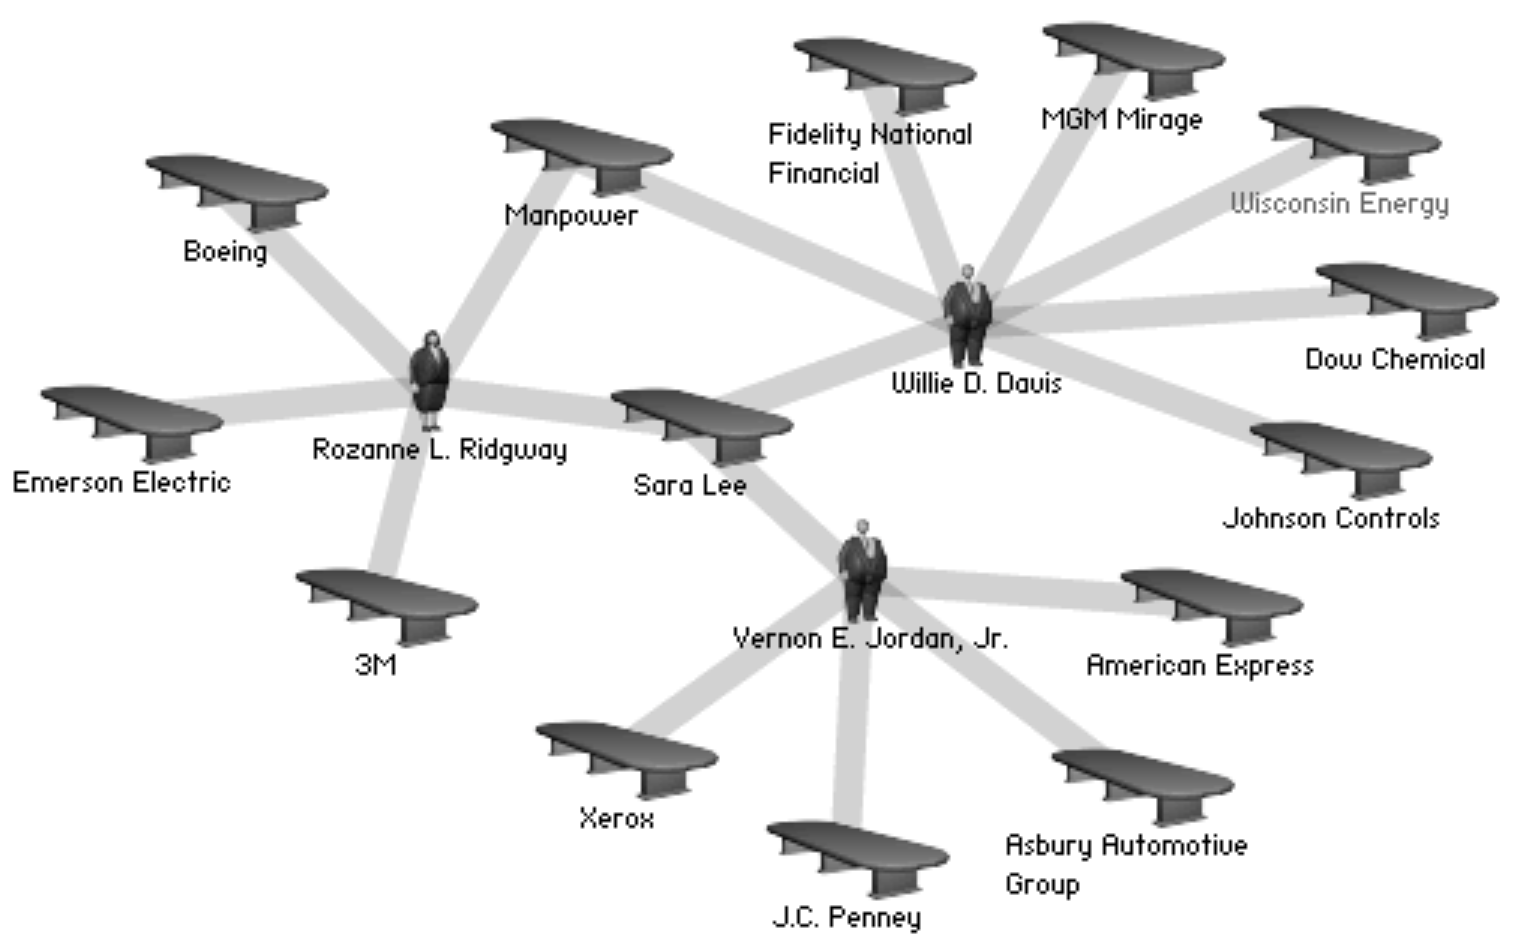
\includegraphics[width=0.8\textwidth]{images/interlock}
			\caption*{A portion of the interlocking directorates
			network connecting US companies.
			\textit{Notes} --- two companies are connected when their at 
			least a boad. \href{https://sites.google.com/site/occupypoliticsintheusa/interlocking-directorates-the-foundation-of-american-corporatocracy}
			{Go to the source.}}
	\end{figure}
\end{frame}

\begin{frame}{Network Density $\rightarrow$ Cooperation}{A simple cooperative game}
	Here is the setup 
	
	\begin{itemize}
		\item Let us have one seller $s$ serving a market with two 
		buyers $b1$ and $b2$
		\item Let us also assume that the parties cannot write a 
		complete contract specifyin the characteristics of the good 
		$s$ sells, say an industrial machinery to produce marmelade 
	\end{itemize}
\end{frame}

\begin{frame}{Network Density $\rightarrow$ Cooperation}{A simple cooperative game}
	\begin{itemize}
		\item Let us have one seller $s$ serving a market with two 
		buyers $b1$ and $b2$
		\item Let us also assume that the parties cannot write a 
		complete contract specifying the characteristics of a `complex' good 
		$s$ sells, say an industrial machinery to produce marmelade 
	\end{itemize}

	\vpsace{1em}

	Does $s$ behave opportunistically by engaging in moral hazard? In other 
	words, does $b$ deliver the good with the agreed features or not?
\end{frame}


\begin{frame}
	{Network Density $\rightarrow$ Cooperation}
	{Let us play the cooperative game together}
	\begin{columns}
	\begin{column}{0.5\textwidth}
		\begin{figure}
				\begin{center}
					%% Creator: Matplotlib, PGF backend
%%
%% To include the figure in your LaTeX document, write
%%   \input{<filename>.pgf}
%%
%% Make sure the required packages are loaded in your preamble
%%   \usepackage{pgf}
%%
%% Also ensure that all the required font packages are loaded; for instance,
%% the lmodern package is sometimes necessary when using math font.
%%   \usepackage{lmodern}
%%
%% Figures using additional raster images can only be included by \input if
%% they are in the same directory as the main LaTeX file. For loading figures
%% from other directories you can use the `import` package
%%   \usepackage{import}
%%
%% and then include the figures with
%%   \import{<path to file>}{<filename>.pgf}
%%
%% Matplotlib used the following preamble
%%   \usepackage{fontspec}
%%   \setmainfont{DejaVuSerif.ttf}[Path=\detokenize{/Users/sbbk475/opt/anaconda3/envs/na/lib/python3.10/site-packages/matplotlib/mpl-data/fonts/ttf/}]
%%   \setsansfont{DejaVuSans.ttf}[Path=\detokenize{/Users/sbbk475/opt/anaconda3/envs/na/lib/python3.10/site-packages/matplotlib/mpl-data/fonts/ttf/}]
%%   \setmonofont{DejaVuSansMono.ttf}[Path=\detokenize{/Users/sbbk475/opt/anaconda3/envs/na/lib/python3.10/site-packages/matplotlib/mpl-data/fonts/ttf/}]
%%
\begingroup%
\makeatletter%
\begin{pgfpicture}%
\pgfpathrectangle{\pgfpointorigin}{\pgfqpoint{2.525000in}{1.740000in}}%
\pgfusepath{use as bounding box, clip}%
\begin{pgfscope}%
\pgfsetbuttcap%
\pgfsetmiterjoin%
\definecolor{currentfill}{rgb}{1.000000,1.000000,1.000000}%
\pgfsetfillcolor{currentfill}%
\pgfsetlinewidth{0.000000pt}%
\definecolor{currentstroke}{rgb}{1.000000,1.000000,1.000000}%
\pgfsetstrokecolor{currentstroke}%
\pgfsetdash{}{0pt}%
\pgfpathmoveto{\pgfqpoint{0.000000in}{0.000000in}}%
\pgfpathlineto{\pgfqpoint{2.525000in}{0.000000in}}%
\pgfpathlineto{\pgfqpoint{2.525000in}{1.740000in}}%
\pgfpathlineto{\pgfqpoint{0.000000in}{1.740000in}}%
\pgfpathlineto{\pgfqpoint{0.000000in}{0.000000in}}%
\pgfpathclose%
\pgfusepath{fill}%
\end{pgfscope}%
\begin{pgfscope}%
\pgfpathrectangle{\pgfqpoint{0.100000in}{0.100000in}}{\pgfqpoint{2.325000in}{1.540000in}}%
\pgfusepath{clip}%
\pgfsetbuttcap%
\pgfsetroundjoin%
\pgfsetlinewidth{1.003750pt}%
\definecolor{currentstroke}{rgb}{0.000000,0.000000,0.000000}%
\pgfsetstrokecolor{currentstroke}%
\pgfsetdash{}{0pt}%
\pgfpathmoveto{\pgfqpoint{1.262500in}{1.506364in}}%
\pgfpathlineto{\pgfqpoint{0.301756in}{0.233636in}}%
\pgfusepath{stroke}%
\end{pgfscope}%
\begin{pgfscope}%
\pgfpathrectangle{\pgfqpoint{0.100000in}{0.100000in}}{\pgfqpoint{2.325000in}{1.540000in}}%
\pgfusepath{clip}%
\pgfsetbuttcap%
\pgfsetroundjoin%
\pgfsetlinewidth{1.003750pt}%
\definecolor{currentstroke}{rgb}{0.000000,0.000000,0.000000}%
\pgfsetstrokecolor{currentstroke}%
\pgfsetdash{}{0pt}%
\pgfpathmoveto{\pgfqpoint{1.262500in}{1.506364in}}%
\pgfpathlineto{\pgfqpoint{2.223244in}{0.233636in}}%
\pgfusepath{stroke}%
\end{pgfscope}%
\begin{pgfscope}%
\pgfpathrectangle{\pgfqpoint{0.100000in}{0.100000in}}{\pgfqpoint{2.325000in}{1.540000in}}%
\pgfusepath{clip}%
\pgfsetbuttcap%
\pgfsetroundjoin%
\definecolor{currentfill}{rgb}{1.000000,1.000000,1.000000}%
\pgfsetfillcolor{currentfill}%
\pgfsetlinewidth{1.003750pt}%
\definecolor{currentstroke}{rgb}{1.000000,1.000000,1.000000}%
\pgfsetstrokecolor{currentstroke}%
\pgfsetdash{}{0pt}%
\pgfsys@defobject{currentmarker}{\pgfqpoint{-0.120281in}{-0.120281in}}{\pgfqpoint{0.120281in}{0.120281in}}{%
\pgfpathmoveto{\pgfqpoint{0.000000in}{-0.120281in}}%
\pgfpathcurveto{\pgfqpoint{0.031899in}{-0.120281in}}{\pgfqpoint{0.062496in}{-0.107608in}}{\pgfqpoint{0.085052in}{-0.085052in}}%
\pgfpathcurveto{\pgfqpoint{0.107608in}{-0.062496in}}{\pgfqpoint{0.120281in}{-0.031899in}}{\pgfqpoint{0.120281in}{0.000000in}}%
\pgfpathcurveto{\pgfqpoint{0.120281in}{0.031899in}}{\pgfqpoint{0.107608in}{0.062496in}}{\pgfqpoint{0.085052in}{0.085052in}}%
\pgfpathcurveto{\pgfqpoint{0.062496in}{0.107608in}}{\pgfqpoint{0.031899in}{0.120281in}}{\pgfqpoint{0.000000in}{0.120281in}}%
\pgfpathcurveto{\pgfqpoint{-0.031899in}{0.120281in}}{\pgfqpoint{-0.062496in}{0.107608in}}{\pgfqpoint{-0.085052in}{0.085052in}}%
\pgfpathcurveto{\pgfqpoint{-0.107608in}{0.062496in}}{\pgfqpoint{-0.120281in}{0.031899in}}{\pgfqpoint{-0.120281in}{0.000000in}}%
\pgfpathcurveto{\pgfqpoint{-0.120281in}{-0.031899in}}{\pgfqpoint{-0.107608in}{-0.062496in}}{\pgfqpoint{-0.085052in}{-0.085052in}}%
\pgfpathcurveto{\pgfqpoint{-0.062496in}{-0.107608in}}{\pgfqpoint{-0.031899in}{-0.120281in}}{\pgfqpoint{0.000000in}{-0.120281in}}%
\pgfpathlineto{\pgfqpoint{0.000000in}{-0.120281in}}%
\pgfpathclose%
\pgfusepath{stroke,fill}%
}%
\begin{pgfscope}%
\pgfsys@transformshift{1.262500in}{1.506364in}%
\pgfsys@useobject{currentmarker}{}%
\end{pgfscope}%
\begin{pgfscope}%
\pgfsys@transformshift{0.301756in}{0.233636in}%
\pgfsys@useobject{currentmarker}{}%
\end{pgfscope}%
\begin{pgfscope}%
\pgfsys@transformshift{2.223244in}{0.233636in}%
\pgfsys@useobject{currentmarker}{}%
\end{pgfscope}%
\end{pgfscope}%
\begin{pgfscope}%
\definecolor{textcolor}{rgb}{0.000000,0.000000,0.000000}%
\pgfsetstrokecolor{textcolor}%
\pgfsetfillcolor{textcolor}%
\pgftext[x=1.262500in,y=1.506364in,,]{\color{textcolor}\sffamily\fontsize{12.000000}{14.400000}\selectfont s}%
\end{pgfscope}%
\begin{pgfscope}%
\definecolor{textcolor}{rgb}{0.000000,0.000000,0.000000}%
\pgfsetstrokecolor{textcolor}%
\pgfsetfillcolor{textcolor}%
\pgftext[x=0.301756in,y=0.233636in,,]{\color{textcolor}\sffamily\fontsize{12.000000}{14.400000}\selectfont b1}%
\end{pgfscope}%
\begin{pgfscope}%
\definecolor{textcolor}{rgb}{0.000000,0.000000,0.000000}%
\pgfsetstrokecolor{textcolor}%
\pgfsetfillcolor{textcolor}%
\pgftext[x=2.223244in,y=0.233636in,,]{\color{textcolor}\sffamily\fontsize{12.000000}{14.400000}\selectfont b2}%
\end{pgfscope}%
\end{pgfpicture}%
\makeatother%
\endgroup%

				\end{center}
				\caption*{Scenario A: an open triad\\$b1$ and $b2$ do not exchange information}
		\end{figure}
	\end{column}
	\begin{column}{0.5\textwidth}
		\begin{figure}
			\begin{center}
				%% Creator: Matplotlib, PGF backend
%%
%% To include the figure in your LaTeX document, write
%%   \input{<filename>.pgf}
%%
%% Make sure the required packages are loaded in your preamble
%%   \usepackage{pgf}
%%
%% Also ensure that all the required font packages are loaded; for instance,
%% the lmodern package is sometimes necessary when using math font.
%%   \usepackage{lmodern}
%%
%% Figures using additional raster images can only be included by \input if
%% they are in the same directory as the main LaTeX file. For loading figures
%% from other directories you can use the `import` package
%%   \usepackage{import}
%%
%% and then include the figures with
%%   \import{<path to file>}{<filename>.pgf}
%%
%% Matplotlib used the following preamble
%%   \usepackage{fontspec}
%%   \setmainfont{DejaVuSerif.ttf}[Path=\detokenize{/Users/sbbk475/opt/anaconda3/envs/na/lib/python3.10/site-packages/matplotlib/mpl-data/fonts/ttf/}]
%%   \setsansfont{DejaVuSans.ttf}[Path=\detokenize{/Users/sbbk475/opt/anaconda3/envs/na/lib/python3.10/site-packages/matplotlib/mpl-data/fonts/ttf/}]
%%   \setmonofont{DejaVuSansMono.ttf}[Path=\detokenize{/Users/sbbk475/opt/anaconda3/envs/na/lib/python3.10/site-packages/matplotlib/mpl-data/fonts/ttf/}]
%%
\begingroup%
\makeatletter%
\begin{pgfpicture}%
\pgfpathrectangle{\pgfpointorigin}{\pgfqpoint{2.525000in}{1.740000in}}%
\pgfusepath{use as bounding box, clip}%
\begin{pgfscope}%
\pgfsetbuttcap%
\pgfsetmiterjoin%
\definecolor{currentfill}{rgb}{1.000000,1.000000,1.000000}%
\pgfsetfillcolor{currentfill}%
\pgfsetlinewidth{0.000000pt}%
\definecolor{currentstroke}{rgb}{1.000000,1.000000,1.000000}%
\pgfsetstrokecolor{currentstroke}%
\pgfsetdash{}{0pt}%
\pgfpathmoveto{\pgfqpoint{0.000000in}{0.000000in}}%
\pgfpathlineto{\pgfqpoint{2.525000in}{0.000000in}}%
\pgfpathlineto{\pgfqpoint{2.525000in}{1.740000in}}%
\pgfpathlineto{\pgfqpoint{0.000000in}{1.740000in}}%
\pgfpathlineto{\pgfqpoint{0.000000in}{0.000000in}}%
\pgfpathclose%
\pgfusepath{fill}%
\end{pgfscope}%
\begin{pgfscope}%
\pgfpathrectangle{\pgfqpoint{0.100000in}{0.100000in}}{\pgfqpoint{2.325000in}{1.540000in}}%
\pgfusepath{clip}%
\pgfsetbuttcap%
\pgfsetroundjoin%
\pgfsetlinewidth{1.003750pt}%
\definecolor{currentstroke}{rgb}{0.000000,0.000000,0.000000}%
\pgfsetstrokecolor{currentstroke}%
\pgfsetdash{}{0pt}%
\pgfpathmoveto{\pgfqpoint{1.262500in}{1.506364in}}%
\pgfpathlineto{\pgfqpoint{0.301756in}{0.233636in}}%
\pgfusepath{stroke}%
\end{pgfscope}%
\begin{pgfscope}%
\pgfpathrectangle{\pgfqpoint{0.100000in}{0.100000in}}{\pgfqpoint{2.325000in}{1.540000in}}%
\pgfusepath{clip}%
\pgfsetbuttcap%
\pgfsetroundjoin%
\pgfsetlinewidth{1.003750pt}%
\definecolor{currentstroke}{rgb}{0.000000,0.000000,0.000000}%
\pgfsetstrokecolor{currentstroke}%
\pgfsetdash{}{0pt}%
\pgfpathmoveto{\pgfqpoint{1.262500in}{1.506364in}}%
\pgfpathlineto{\pgfqpoint{2.223244in}{0.233636in}}%
\pgfusepath{stroke}%
\end{pgfscope}%
\begin{pgfscope}%
\pgfpathrectangle{\pgfqpoint{0.100000in}{0.100000in}}{\pgfqpoint{2.325000in}{1.540000in}}%
\pgfusepath{clip}%
\pgfsetbuttcap%
\pgfsetroundjoin%
\pgfsetlinewidth{1.003750pt}%
\definecolor{currentstroke}{rgb}{0.000000,0.000000,0.000000}%
\pgfsetstrokecolor{currentstroke}%
\pgfsetdash{}{0pt}%
\pgfpathmoveto{\pgfqpoint{0.301756in}{0.233636in}}%
\pgfpathlineto{\pgfqpoint{2.223244in}{0.233636in}}%
\pgfusepath{stroke}%
\end{pgfscope}%
\begin{pgfscope}%
\pgfpathrectangle{\pgfqpoint{0.100000in}{0.100000in}}{\pgfqpoint{2.325000in}{1.540000in}}%
\pgfusepath{clip}%
\pgfsetbuttcap%
\pgfsetroundjoin%
\definecolor{currentfill}{rgb}{1.000000,1.000000,1.000000}%
\pgfsetfillcolor{currentfill}%
\pgfsetlinewidth{1.003750pt}%
\definecolor{currentstroke}{rgb}{1.000000,1.000000,1.000000}%
\pgfsetstrokecolor{currentstroke}%
\pgfsetdash{}{0pt}%
\pgfsys@defobject{currentmarker}{\pgfqpoint{-0.120281in}{-0.120281in}}{\pgfqpoint{0.120281in}{0.120281in}}{%
\pgfpathmoveto{\pgfqpoint{0.000000in}{-0.120281in}}%
\pgfpathcurveto{\pgfqpoint{0.031899in}{-0.120281in}}{\pgfqpoint{0.062496in}{-0.107608in}}{\pgfqpoint{0.085052in}{-0.085052in}}%
\pgfpathcurveto{\pgfqpoint{0.107608in}{-0.062496in}}{\pgfqpoint{0.120281in}{-0.031899in}}{\pgfqpoint{0.120281in}{0.000000in}}%
\pgfpathcurveto{\pgfqpoint{0.120281in}{0.031899in}}{\pgfqpoint{0.107608in}{0.062496in}}{\pgfqpoint{0.085052in}{0.085052in}}%
\pgfpathcurveto{\pgfqpoint{0.062496in}{0.107608in}}{\pgfqpoint{0.031899in}{0.120281in}}{\pgfqpoint{0.000000in}{0.120281in}}%
\pgfpathcurveto{\pgfqpoint{-0.031899in}{0.120281in}}{\pgfqpoint{-0.062496in}{0.107608in}}{\pgfqpoint{-0.085052in}{0.085052in}}%
\pgfpathcurveto{\pgfqpoint{-0.107608in}{0.062496in}}{\pgfqpoint{-0.120281in}{0.031899in}}{\pgfqpoint{-0.120281in}{0.000000in}}%
\pgfpathcurveto{\pgfqpoint{-0.120281in}{-0.031899in}}{\pgfqpoint{-0.107608in}{-0.062496in}}{\pgfqpoint{-0.085052in}{-0.085052in}}%
\pgfpathcurveto{\pgfqpoint{-0.062496in}{-0.107608in}}{\pgfqpoint{-0.031899in}{-0.120281in}}{\pgfqpoint{0.000000in}{-0.120281in}}%
\pgfpathlineto{\pgfqpoint{0.000000in}{-0.120281in}}%
\pgfpathclose%
\pgfusepath{stroke,fill}%
}%
\begin{pgfscope}%
\pgfsys@transformshift{1.262500in}{1.506364in}%
\pgfsys@useobject{currentmarker}{}%
\end{pgfscope}%
\begin{pgfscope}%
\pgfsys@transformshift{0.301756in}{0.233636in}%
\pgfsys@useobject{currentmarker}{}%
\end{pgfscope}%
\begin{pgfscope}%
\pgfsys@transformshift{2.223244in}{0.233636in}%
\pgfsys@useobject{currentmarker}{}%
\end{pgfscope}%
\end{pgfscope}%
\begin{pgfscope}%
\definecolor{textcolor}{rgb}{0.000000,0.000000,0.000000}%
\pgfsetstrokecolor{textcolor}%
\pgfsetfillcolor{textcolor}%
\pgftext[x=1.262500in,y=1.506364in,,]{\color{textcolor}\sffamily\fontsize{12.000000}{14.400000}\selectfont s}%
\end{pgfscope}%
\begin{pgfscope}%
\definecolor{textcolor}{rgb}{0.000000,0.000000,0.000000}%
\pgfsetstrokecolor{textcolor}%
\pgfsetfillcolor{textcolor}%
\pgftext[x=0.301756in,y=0.233636in,,]{\color{textcolor}\sffamily\fontsize{12.000000}{14.400000}\selectfont b1}%
\end{pgfscope}%
\begin{pgfscope}%
\definecolor{textcolor}{rgb}{0.000000,0.000000,0.000000}%
\pgfsetstrokecolor{textcolor}%
\pgfsetfillcolor{textcolor}%
\pgftext[x=2.223244in,y=0.233636in,,]{\color{textcolor}\sffamily\fontsize{12.000000}{14.400000}\selectfont b2}%
\end{pgfscope}%
\end{pgfpicture}%
\makeatother%
\endgroup%

			\end{center}
			\caption*{Scenario B: a closed triad\\$b1$ and $b2$ exchange information}
	\end{figure}
	\end{column}
	\end{columns}
\end{frame}

\begin{frame}
	{Network Density $\rightarrow$ Trust}
	{Why do we trust `places' as well as `businesses'?}
        \begin{figure}
        	\begin{center}
        		
\includegraphics[width=0.9\textwidth]{images/trust_research.png}
        	\end{center}
        \end{figure}
\end{frame}

% =========================== Measuring network density =====================
\section{Measuring Density}

\begin{frame}{Density Metrics}
	\begin{tcolorbox}[
		colback=comp_c!5!white,
		colframe=comp_c!90!black,
		title={\centering !! Pay attention !!}]
		There is no single metric capturing the concept of network density
	\end{tcolorbox}

	\vspace{2em}

	In practice, we use complementary metrics such as 

	\begin{itemize}
		\item Average degree 
		\item Degree distribution 
		\item Connectdeness
		\item Clustering coefficient
	\end{itemize}
\end{frame}

% =========================== Bibliography =================================
\begin{frame}
	\frametitle{References}
	\printbibliography
 \end{frame} 

% =========================== Document end ================================== 
\end{document}